\documentclass[thesis.tex]{subfiles}
\begin{document}
\chapter{Instantiating and Evaluating SecPAL}
\label{chap:apppal}

\begin{figure}
  \centering\noindent
  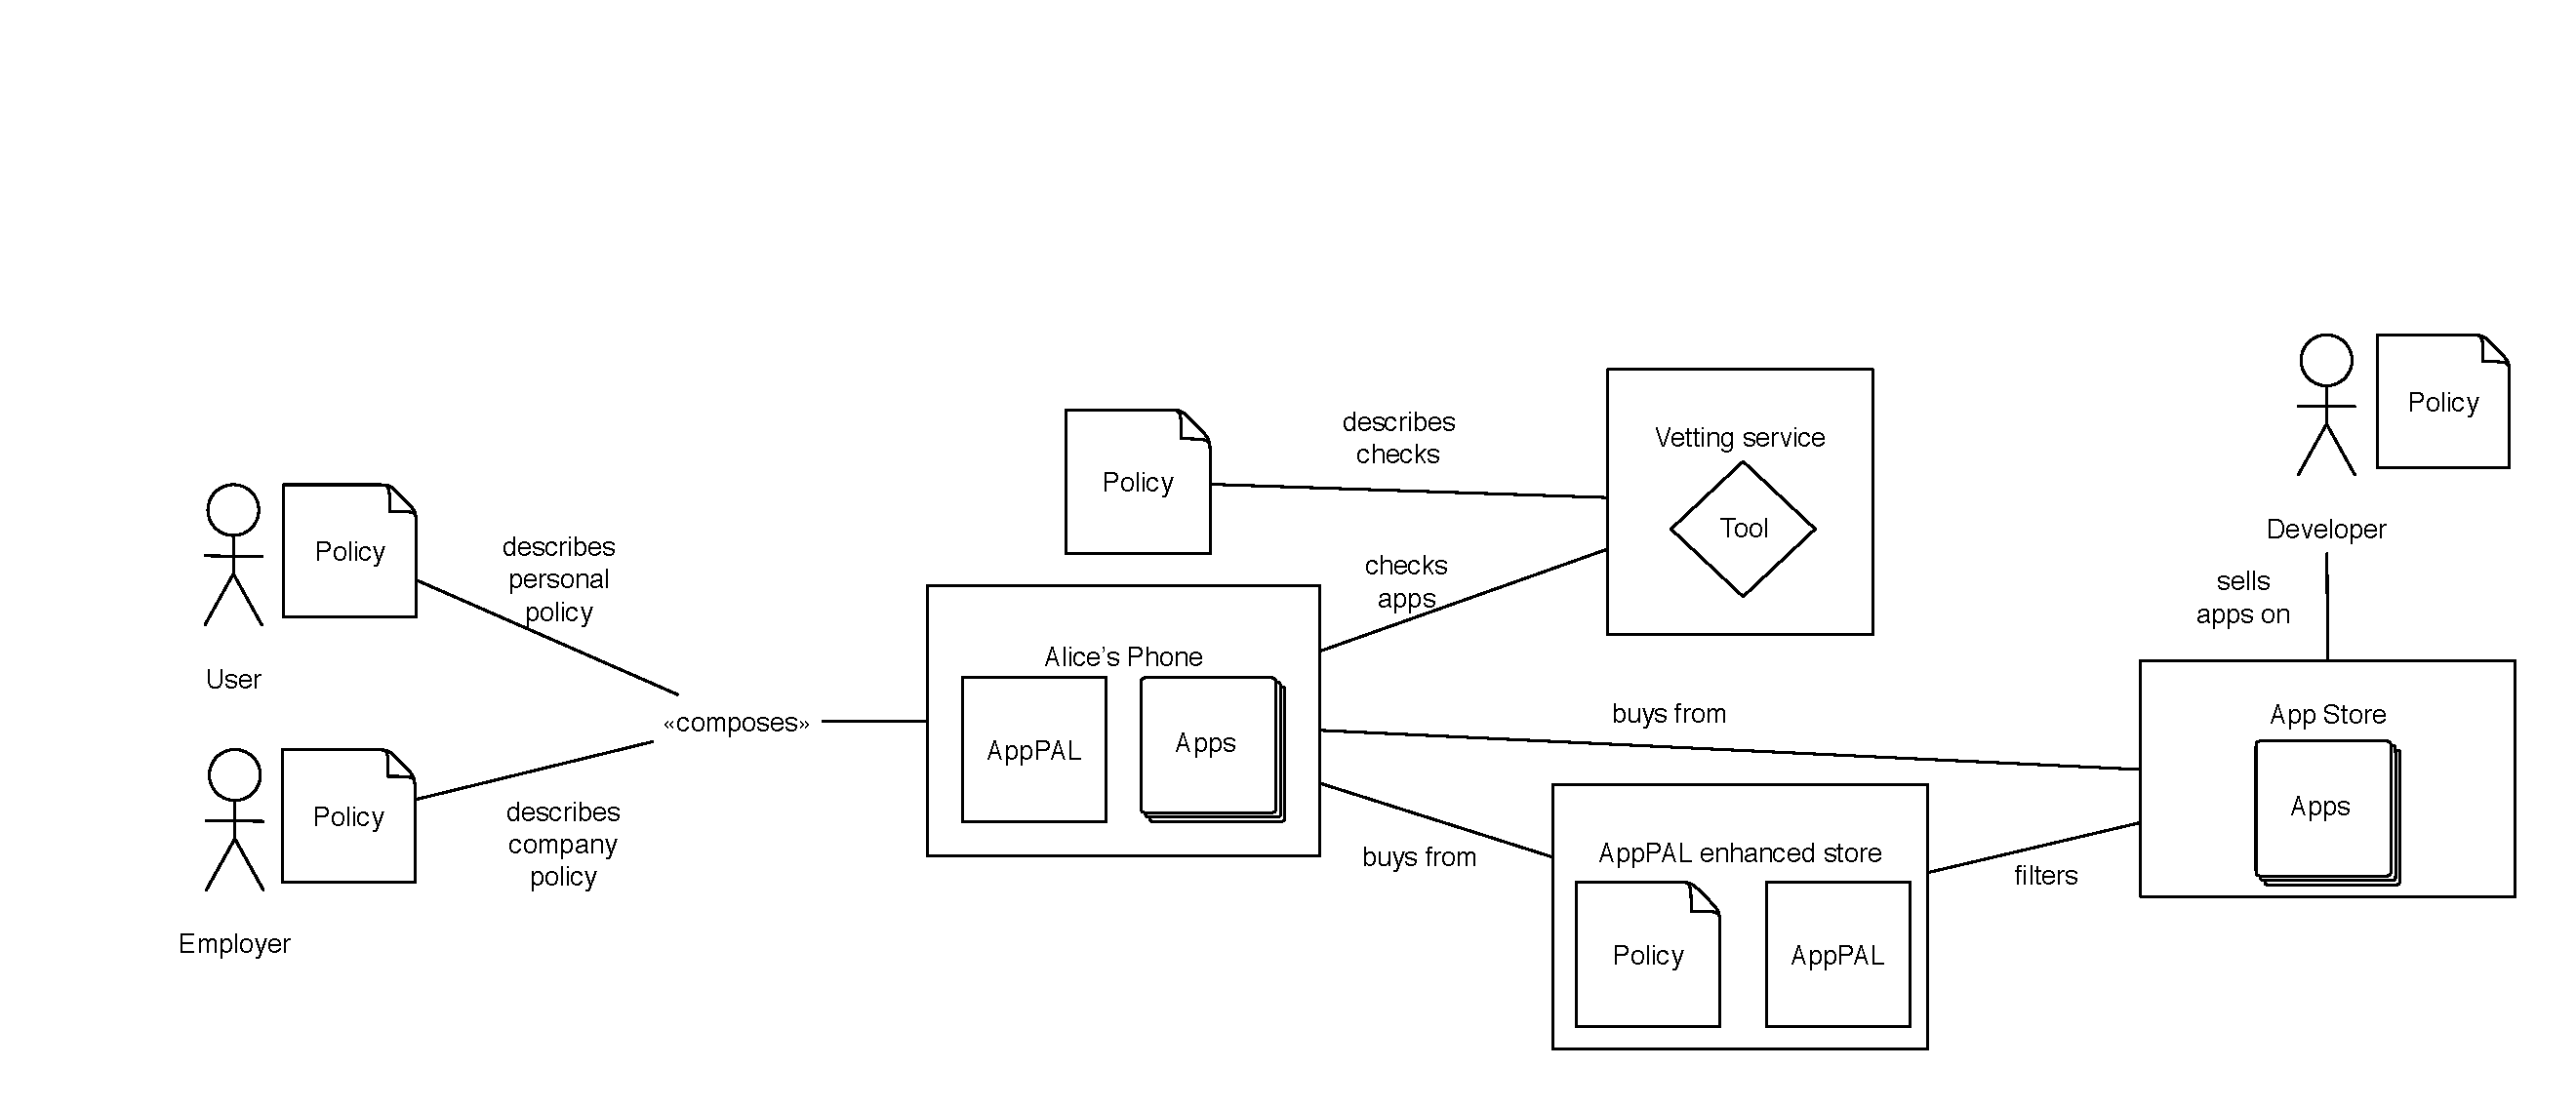
\includegraphics[width=\textwidth]{figures/policies-ecosystem.pdf}
  \medskip
  \caption[Entities in the mobile ecosystem]{Entities in the mobile ecosystem
    and some of the policies surrounding them.}
  \label{fig:ecosystem}
\end{figure}

The mobile ecosystem (which we define as the devices, users, stores,
developers and policies surrounding the ways we use mobile devices)
contains many interacting entities, including devices interacting with
their users, app stores selling software, developers building apps,
wireless access points devices connect to, and the companies and
networks the devices and their users work within.

Every entity in the ecosystem has its own policies. For example, there
is a contract between the store selling apps and the developer
programming them. The stores have content policies as to which apps
they will sell, often prohibiting sexual or illicit content. The app
developers may have preferences as to which stores they will sell
their apps in, favouring stores with higher market shares, or which
take smaller cuts of the app sale price. Not all policies are as
formal as a contract: a user may have preferences about which kinds of
apps he wants to install but may not write these preferences down.
Instead, he might pick apps to install from a store based on his best
guess whether it matches his preferences. The mobile ecosystem is a
\emph{distributed system}. Phones, users and stores are not aware of
each other until they interact---there is no list of every app store,
every device and every user.  They must make policy decisions on their
own without relying on a central authority to make decisions for
them. They can, if required, delegate to others for their policies and
knowledge.

Formal languages let us write policies without ambiguity and describes
precisely the process behind making decisions. A policy written in a
formal language describes what decisions can be made. Translating
policies into a formal language allows for rigorous comparisons of
different policies, preferences and rules in mobile
ecosystems. Writing the policy in a formal language gives a precise
meaning and \emph{perhaps} allows it to be checked automatically, if
the policy is decidable.

Becker~et~al{.} designed SecPAL to make access control decisions in
distributed systems~\cite{becker_secpal:_2006}. SecPAL is expressive,
has a clear and intuitive syntax, is decidable and extensible. That
SecPAL is extensible is important as we can apply the language to a
new domain by instantiating it with predicates and constraints.

This chapter introduces how SecPAL is instantiated to describe the
policies surrounding mobile ecosystems. We explain why SecPAL is a
good choice to describe policies in the mobile ecosystem. I introduce
AppPAL as an instantiation and implementation of SecPAL for mobile
device policies.


\section{Why SecPAL}
\label{sec:why-apppal}

There are many policy languages. Some target specific domains: such as
Ponder which targets firewalls, OS's and
databases~\cite{damianou_ponder_2001}. Others, such as Cassandra,
focus on credential management~\cite{becker_cassandra:_2004}.  Some
are general like XACML~\cite{oasis_extensible_2013}: designed to
express access control decisions from a variety of domains. Different
policy languages are described in greater detail in
\autoref{chap:background}.

The mobile ecosystem has specific requirements for a policy language
to describe its policies. Namely, we need a policy language that can
express:

\begin{description}
  \item[Delegation.] Sometimes entities may wish to
    share information and policy rules. A user might delegate to an
    expert user to help them decide what policies they want to use. An app
    store might use information from an app vetting firm to decide what
    apps to sell. A company might want HR and IT departments to be
    responsible for some decisions, and they in turn might wish to give
    specific HR or IT workers specific decisions to make. Capturing these
    relationships lets us describe precisely who makes what decisions in
    the mobile ecosystem.

  \item[Locality.] In the mobile ecosystem different devices can have different
    policies. For example, two users of mobile phones may disagree about what
    makes an app \emph{installable} (i{.}e{.}~acceptable to install). Equally,
    the policies a store may wish to enforce are very different from the policies
    a user may wish to enforce. The locality of a query is the place where the
    decision is being made, typically in the immediate vicinity of an entity such
    as a user or store. Each entity in the ecosystem also expects to enforce
    their own policies---there is no overarching enforcer of policies, rather
    users enforce whatever preferences they have, stores enforce their own rules
    through whatever means they see fit. Being able to point to the location a
    decision is made is important when considering delegation: a user might ask a
    friend if an app is good: we want to distinguish between the friend telling
    the user directly, and the friend giving the user sufficient information to
    draw the conclusion themselves.

  \item[Access external information.] There are many tools and sources
    that can give us information about apps (as well as other
    subjects). These tools each give information in their own way: be it
    employee data through an SQL database, terminal output through a
    command line analysis tool, or HTML output onto an app store's
    web-page. We want to be able to make use of this information when
    writing policies, but we should not rely on all tools standardising on
    our policy language as a universal information transfer mechanism. We
    want our policy language to be able to capture the policies which use
    these external sources without forcing the tools themselves to work in
    any particular manner. In other words, the policy \emph{specification
    should be separate from its enforcement}.

  \item[Constraints.] As well as external information, we'd also wish
    our policy language to capture dynamic information such as the time of
    day or the current location of a device. This information is sometimes
    incorporated into a policy language through \emph{constraints}. This
    would allow us to start to create rules that depend on the context of
    the user. For example a company boss might want to check what time
    their employees get into work. To do this the boss requires their
    employees install an app that gives him their location. Employees
    might allow their boss to check on them during the work day, but
    during the weekend and the evenings the employee would rather their
    boss could not see where they were.

  \item[Flexibility of Policy Style.] The mobile ecosystem encompasses
    many scenarios. A company looking to enforce a mobile device
    policy would use a MAC-style policy, but a user trying to filter what
    APIs an app can access may write a policy in a DAC-style. A user
    trying to describe might be happy to install an app with certain
    permissions if the app has a particular purpose. For example a user
    might be happy to install a file management app that can access a
    memory card, but not happy to install a torch app with the same set
    of permissions---a policy reminiscent of an RBAC or ABAC policy. We
    want to capture all these policies, and we would want our policy
    language to be agnostic to any particular policy style.
\end{description}

We chose SecPAL as the basis for our policy language for mobile ecosystems as it
provides the features we wanted. By using its \emph{can-say} and
\emph{can-act-as} phrases we can capture different delegation patters (as
described in~\autoref{ssec:delegation_in_secpal}).

Every assertion in SecPAL is made by an explicit speaker, who should sign each
statement with a key. This gives locality to statements. If we have an assertion
from Alice that she thinks an app is good then it must have come directly from
Alice. If we just have assertions from Alice that describe the general process
for deciding if an app is good or not, then we might reasonably believe that the
decision whether Alice would consider an individual app good or not might
be made elsewhere.

SecPAL's constraint mechanism (the \emph{where} part of an assertion) lets us
implement the constraints we described but also allows us to access external
information. Constraint functions can be written to run a particular tool, or
make a query to a database, allowing us access to external information.

SecPAL policies are style agnostic, and the language does not
prescribe a particular style to write polices in.
It is easy to capture idiomatic policy styles using SecPAL.  For example, a classic example of a DAC-style policy are UNIX file permissions.  
The decision by an OS whether to allow a user (U) to read a file (F) based on the permissions on the file-system (FS) can be written in SecPAL:
\begin{lstlisting}
'os' says User:U canRead(File:F)
  if F hasOwner(U),
     F hasPermissionsMask('400').

'os' says User:U canRead(File:F)
  if F hasGroup(G),
     U isMemberOf(G),
     F hasPermissionsMask('040').

'os' says User:U canRead(File:F)
if F hasPermissionsMask('004').

'os' says 'fs' can-say File:F hasOwner(User:U).
'os' says 'fs' can-say File:F hasPermissionsMask(Mask:M).
\end{lstlisting}
Similarly, we can also capture the \emph{simple} and
\emph{star} MAC rules of the Bell-LaPadula model (the \emph{read-down,
write-up} rules) using SecPAL:
\begin{lstlisting}
'admin' says User:U canRead(File:F)
  if U isSecurityLevel(LU),
     F isSecurityLevel(LF)
  where LU >= LF.

'admin' says User:U canWrite(File:F)
  if U isSecurityLevel(LU),
     F isSecurityLevel(LF)
  where LU <= LF.
\end{lstlisting} Writing RBAC, or ABAC-style policies is similarly
easy.  Unlike some languages, such as Cassandra~\cite{becker_cassandra:_2004} or RT~\cite{li_design_2002}, which encourage
a certain style of policy, SecPAL doesn't say \emph{how} a policy
should be written, it instead lets the policy author write their rules
as they see best.

As well meeting our requirements for a policy language, we agree with
Becker~\etal's assertion that SecPAL is readable and has evaluation
rules that are easy to understand and
unsurprising~\cite{becker_secpal:_2006}.  This again makes SecPAL a
good fit to describe the policies of the mobile ecosystem as even
someone unfamiliar with SecPAL might be able to look at an assertion
and be reasonably expected to understand what the assertion means.

Tschantz and Krishnamurthi defined various reasonability properties
(properties that determine how well someone might predict how a policy
will behave) for policy
languages~\cite{tschantz_towards_reasonability_2006}.  They note that
compared to languages based on first-order logic (like SecPAL):
\begin{quotation}
  ``policies written in XACML are more transparent than policies written in languages based on first-order logic''
\end{quotation} In their paper, Tschantz and Krishnamurthi compare a
restricted version of XACML (Core XACML) to three first-order logic
based languages: FOL, Lithium and $\mathcal{L}_5$.  Tschantz and
Krishnamurthi go on to define their properties: \emph{totality} if the
language always makes a decision, \emph{determinism} if the language
always makes the same decision given the same query, \emph{monotonic}
if the policy makes the same decisions if the rules are reordered,
\emph{safety} if adding a facts from a policy only allows more permit
decisions to be made and \emph{independent composition} if the results
of querying the policy as a whole are no different from querying
subsets of the policy's rules and combining them.  They note that
whilst Core XACML is deterministic it is not safe, does not have
independent composition and is not monotonic.

SecPAL in contrast is total (by the closed world assumption), is
monotonic (there are no policy combinators and negation is not allowed
in policies), and has independent composition (there are no policy
combinators).  If the policy is always structured to use the same form
of decision (the policy always uses \texttt{canRead} instead of
\texttt{canNotRead}, for example) then the language is safe too.
SecPAL without constraints is also deterministic, and if constraints
are used then the language is deterministic only if the constraints
themselves are\footnote{A constraint which rolled a dice and checked
if the number rolled was 2 would not be deterministic but could be
used in SecPAL.}.  SecPAL seems, therefore, to meet most of Tschantz
and Krishnamurthi criteria for a reasonable language, despite being
based of first-order logic.

Other languages, perhaps such as XACML or Ponder, could have been used as a
starting point for a policy language. We chose SecPAL, however, as the basis for
AppPAL---a policy language for mobile ecosystems.

\section{Basic Examples of AppPAL}

AppPAL is a policy language that describes the policies of the mobile
ecosystem.  To be more precise: it is SecPAL, with a slightly modified
syntax to allow for additional typing constraints (described
in~\autoref{ssec:types}) and to aid machine parsing.  As well as the
modified syntax, AppPAL also instantiates SecPAL (which is generic) to
with the predicates and types to talk about mobile security policies
(\autoref{sec:instantiating}).

One example of the policies AppPAL might describe is a user selecting
which apps they want to use on their phone. Suppose a user, Alice,
decides that an individual app (Angry Birds, for example) is okay to
use on her phone. This is written as:

\begin{lstlisting}
'alice' says 'com.rovio.angrybirds' isInstallable.
\end{lstlisting} Having decided the app is the one Alice wishes to use she tells
the device's package manager that it must install the app. The package manager
might be connected to an app store (such as the Play Store on Android: the
\texttt{com.android.vending} APK file), a \ac{MDM} program such as iOS's
\ac{VPP}, or an IT manager manually provisioning devices. The user may not know
who fills the role of the \emph{package manager} but most systems provide one
nevertheless.
\begin{lstlisting}
'alice' says 'package-manager'
  mustInstall ('com.rovio.angrybirds').
'alice' says 'com.android.vending' can-act-as 'package-manager'.
\end{lstlisting}
Additionally Alice may allow her workplace to dictate some apps that must be installed (a delegation).
\begin{lstlisting}
'workplace' says 'alice' mustInstall('com.microsoft.office.word').
'alice' says 'workplace' can-say
  'alice' mustInstall('com.microsoft.office.word').
\end{lstlisting}
This policy works with single apps: Alice decides which apps to
install and lists them.  This is an accurate description of how users
currently interact with stores and their devices.  Users may have more
complicated rules for deciding what to install, but following the
rules is usually left to the user's own self-discipline.

Policy languages allow for greater generality.  A cautious user may
only install Android apps with certain
permissions\footnote{Permissions are the access control mechanism for
  device features used by Android.}.
\begin{lstlisting}
'user' says App isInstallable
  if App hasntPermission('CAMERA'),
     App hasntPermission('INTERNET'),
\end{lstlisting}
Others may avoid apps that allow them to spend money within the app.
\begin{lstlisting}
'user' says App isInstallable
  if App cannotMakeInAppPurchases.
\end{lstlisting}
Some users may rely on an \ac{AV} program installed on their phone.
The phone can only install apps checked by the \ac{AV} program.
\begin{lstlisting}
'user' says App:A isInstallable
  where runAV(A) = 'safe'.
\end{lstlisting}
Alternatively a user may allow an app to be installed if two or more of their friends are willing to recommend the app to them.
\begin{lstlisting}
'user' says App isInstallable
  if App isRecommendedBy(Friend1),
     App isRecommendedBy(Friend2)
  where Friend1 != Friend2.

'user' says Friend:F can-say
  App:A isRecommendedBy(F).
\end{lstlisting}


\subsection{AppPAL Policies for App Stores}
AppPAL gives a language for describing these decision-making processes. By
writing down policies in formal language we not only start to allow
machine-based decision-making, avoiding the need for user's self-control, but we
also can compare different policies. This goes beyond describing user's app
preferences. Consider the two largest mobile operating systems: Apple's iOS and
Google's Android. When comparing the systems Apple's is often described as a
\emph{walled-garden} whereas Android is an
\emph{open-platform}~\cite{barrera_secure_2011,enck_defending_2011}. Language
like this is informal. It hints at the differences without giving them
precisely.

Using AppPAL we can model the differences between the two systems and make more
meaningful comparisons. The \emph{walled-garden} comments relate to their
different app store models. Users of iOS can only install apps from the \emph{App
Store}\footnote{\emph{The App Store} is Apple's marketplace for selling apps, an
\emph{app store} is a generic term for an on-device store selling apps.}. If a
user is willing to install a special certificate, from a developer or business,
however they may install apps through the browser or a computer connected to the
device. Apple controls these special certificates, issuing and revoking them.
They must also be authorised by the device's owner.
\begin{lstlisting}
'device' says App isInstallable
  if App hasBeenSignedBy(Cert),
     Cert hasIssuer('apple').

'device' says App isInstallable
  if App hasBeenSignedBy(Cert),
     Cert hasIssuer(X),
     'apple' hasAuthorized(X),
     'device' hasOwner(U),
     U hasAuthorized(Cert)
  where validCertificate(App, Cert) = true.

'device' says Authority:A can-say A hasAuthorized(Certificate:C).
\end{lstlisting}
In contrast, an Android user is free to install any signed app (though
who signed it is not immediately important).  Unless the user has
enabled \emph{side-loading}, the app must come from the Play Store, as
opposed to a file downloaded through another app store or the
internet.  Alternatively, if the user has enabled
\emph{developer-mode} then they may install apps through the \ac{ADB}.

\noindent\begin{minipage}{\textwidth}\vspace{1em}
\begin{lstlisting}
'device' says App isInstallable
  if App hasSource('play-store'),
     App hasBeenSignedBy(Cert)
  where validCertificate(App, Cert) = true.

'device' says App isInstallable
  if App hasSource('file')
     'device' hasOwner(U),
     U hasAuthorized('sideloading'),
     App hasBeenSignedBy(Cert)
  where validCertificate(App, Cert) = true.
\end{lstlisting}
\end{minipage}

\noindent\begin{minipage}{\textwidth}
\begin{lstlisting}
'device' says 'settings-app' can-say
  U hasAuthorized('sideloading').

'device' says App isInstallable
  if App hasSource('adb')
     'device' hasOwner(U),
     U hasAuthorized('developer-mode').

'device' says 'settings-app' can-say
  U hasAuthorized('developer-mode').

'settings-app' says 'user' can-say
  'user' hasAuthorized(Setting:X).
\end{lstlisting}
\end{minipage}

This glosses over some details of certificate handling (though the
example could be extended further). It also ignores how the system might update
apps. It does, however, provide a far more precise version of the differences in
app installation between the two platforms. For iOS, to install an app Apple
have to authorise it, either by signing the app or the issuer. In contrast, for
Android, to the device can install any app if the device owner is willing to
enable the relevant setting.

\subsection{Worked Example of Policy Checking}

As a worked example consider a user Alice, trying to install an app on
her work phone.  Alice works for a hospital trust and the trust has a
mobile device policy.  The trust's policy states that if Alice wants to
install an app Alice has to clear it with her immediate manager.  If
it is for clinical use then Alice also has to clear it with the
\ac{CACPG}.  If it is for business use then Alice also has to clear it
with the \ac{MIG}.  Finally, the \ac{IGC} should clear the app.  This
is a relatively complicated policy but realistic: it comes from an
actual NHS trust's BYOD rules (shown with an AppPAL translation in
\autoref{appendix:byod}).

To implement the policy the trust publishes the following AppPAL rules:

\noindent\begin{minipage}{\textwidth}
\begin{lstlisting}
'nhs-trust' says App isUsable
  if App hasMet('clinical-use-case').

'nhs-trust' says App isUsable
  if App hasMet('business-use-case').

'nhs-trust' says 'cacpg' can-say
  App:A hasMet('clinical-use-case').

'nhs-trust' says 'mig' can-say
  App:A hasMet('business-use-case').

'nhs-trust' says App isInstallable
  if App hasMet('final-app-approval'), App isUsable.

'nhs-trust' says 'igc' can-say
  App hasMet('final-app-approval').

'nhs-trust' says Device canInstall(App)
  if App isInstallable, App isApprovedFor(Device).

'nhs-trust' says Employee:Manager can-say
  App:A isApprovedFor(Device)
  if Manager isResponsibleFor(Device).
\end{lstlisting}
\end{minipage}

Suppose Alice wishes to install the app \emph{\ttfamily ms.office} for
business purposes.  To satisfy the policy and install the app she
needs to collect the following statements.

\begin{itemize}
    %\newand{\weitemsize}[0]{\footnotesize}
  \item \lstinline!'nhs-trust' says 'ms.office' isInstallable.!
    For this, she needs the \ac{MIG} to state that it has a business use-case.
    She also needs approval from the \ac{IGC}.
    \begin{enumerate}\setcounter{enumi}{0}
      \item \lstinline!'mig' says 'ms.office' hasMet('business-use-case').!
      \item \lstinline!'igc' says 'ms.office' hasMet('final-app-approval').!
    \end{enumerate}
  \item \lstinline!'nhs-trust' says 'ms.office' isApprovedFor('alices-device').!

    To get this she needs a statement from the manager responsible for Alice's device (suppose it is \emph{Bob}) approving the app.
    \begin{enumerate}\setcounter{enumi}{2}
      \item \lstinline!'bob' says 'ms.office' isApprovedFor('alices-device').!
      \item \lstinline!'nhs-trust' says 'bob' isResponsibleFor('alices-device').!
    \end{enumerate}
  \item Additionally, she needs the following typing statements.
    \begin{enumerate}\setcounter{enumi}{4}
      \item \lstinline!'nhs-trust' says 'ms.office' isApp.! \label{item:isapp}
      \item \lstinline!'nhs-trust' says 'bob' isEmployee.!
    \end{enumerate}
\end{itemize}

\noindent Alice obtains the statements by contacting the speakers. Each may either give
her the statement she needs or may give her more rules in the form of a
cryptographically signed electronic representation of each assertion. For
the \ac{MIG} and \ac{IGC} may authorise the app or they might give a
list of additional checks they need before they agree to authorise the app. When
checking if the app is an App in \autoref{item:isapp}, the NHS trust might
delegate further. They could reply that if the App is in the Google Play store
then they recognise it as a valid app. Alice would then have to get more
assertions if she wanted to prove this statement. Alternatively, the speaker
could refuse to make the assertion, either because they do not believe it, or
they cannot give an answer. In this case, Alice would have to look for an
alternative means to prove the assertion or accept that they cannot install the
app.

Once Alice has collected the statements, either by contacting the speakers
directly or through other means, Alice can use a SecPAL inference tool, such as
AppPAL, to check whether she can install the app. Additional to the decision, if
a proof is found, a tool like AppPAL can output a proof
tree\footnote{Technically a DAG.} to show how it made the decision
(\autoref{fig:exemplar-proof}). The proof tree shows the AppPAL assertions used
to prove each statement at varying levels of the tree: from the top-level
goal which, in this case, used the \emph{cond} rule first shown in \autoref{fig:secpal-rules}.

\begin{center}
  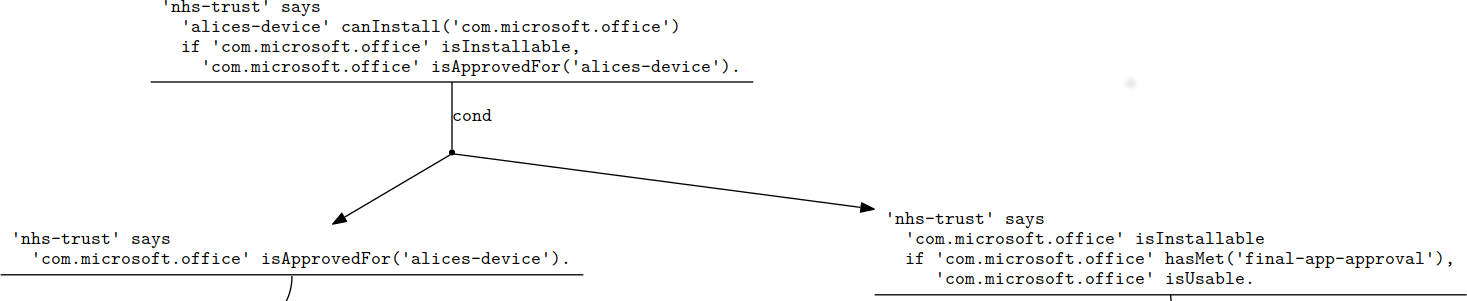
\includegraphics[width=0.9\linewidth]{figures/exemplar-proof-1.png}
\end{center}

To later nodes which might use SecPAL's other rules to be proved (\emph{can-say} in this case).

\begin{center}
  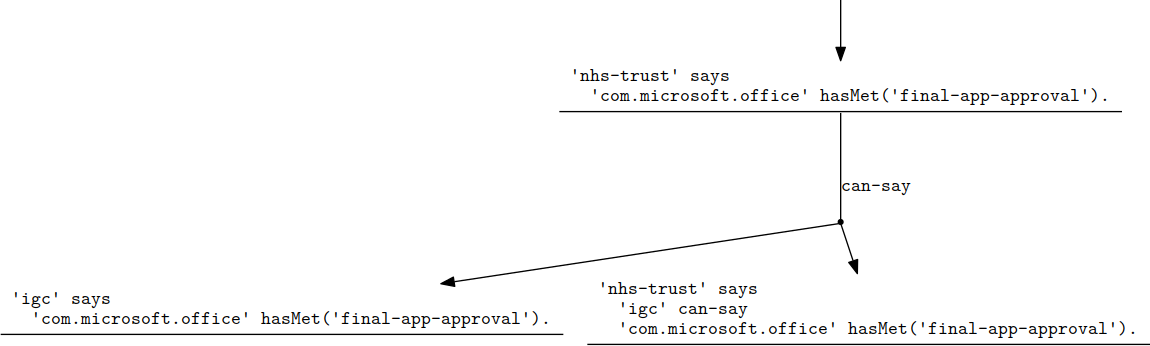
\includegraphics[width=0.9\linewidth]{figures/exemplar-proof-2.png}
\end{center}

If two nodes depend on the same sub-goals, then the proof will be reused.

\begin{center}
  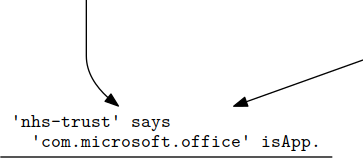
\includegraphics[width=0.3\linewidth]{figures/exemplar-proof-3.png}
\end{center}

\begin{figure}
  \centering
  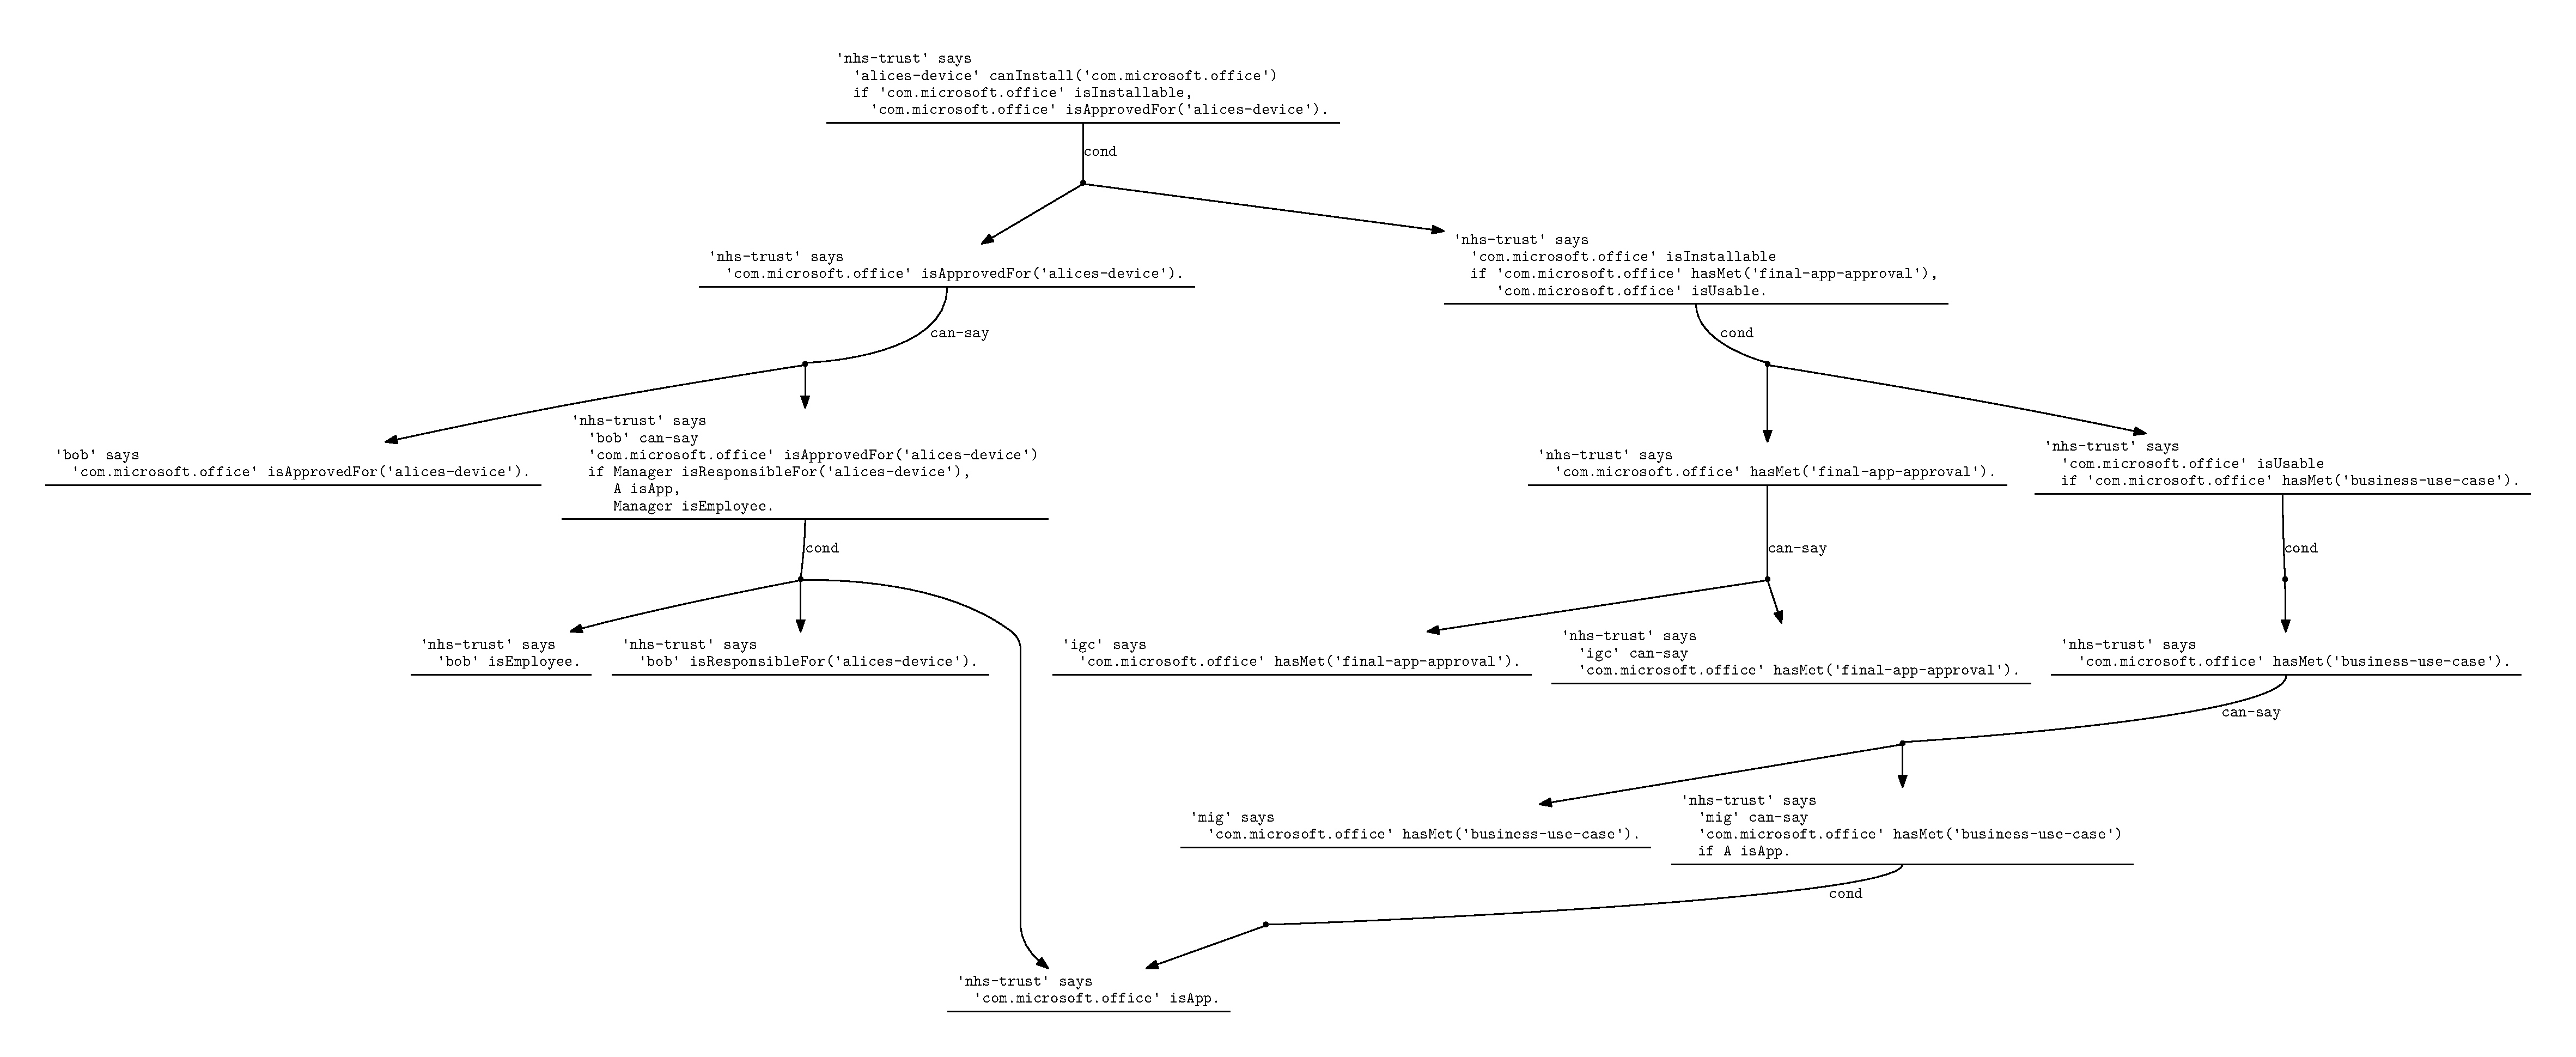
\includegraphics[width=0.9\textheight, angle=90]{figures/exemplar-proof.pdf}
  \caption[Proof tree output by AppPAL.]{Proof tree generated by AppPAL when checking whether to install Alice's app.}
  \label{fig:exemplar-proof}
\end{figure}

\section{Instantiating SecPAL for Mobile Ecosystems}
\label{sec:instantiating}

SecPAL is a generic language.  In SecPAL's
grammar~(\autoref{fig:secpal-grammar}), predicates and constraint
functions describe the decisions and checks done in a particular
domain.  The choice of predicates and constraints defines the
decisions the SecPAL instantiation can talk about.

AppPAL instantiates SecPAL to describe policies in mobile
ecosystems. It was initially focused on
describing app installation policies, however it was later extended
further to describe other policies, such as \ac{BYOD} policies.

\subsection{Predicate Conventions}
\label{ssec:predicate-conventions}

\newcommand{\descPred}[2]{\emph{subject} \texttt{\textbf{#1}\emph{#2}}}
\begin{table}\footnotesize\sffamily\centering
  \begin{tabular}{l l}
    \toprule
    Prefix                      & Meaning                                            \\
    \midrule
    \descPred{can}{Action}      & The subject is allowed to perform the action.      \\
    \descPred{has}{Action}      & The subject has performed the action.              \\
    \descPred{is}{Property}     & The property holds true for the subject.           \\
    \descPred{must}{Obligation} & The subject is required to satisfy the obligation. \\
    \bottomrule
  \end{tabular}
  \caption{Standard prefixes used for AppPAL predicates.}
  \label{tab:predicate-prefixes}
\end{table}

When instantiating SecPAL we use predicates based on four verbs: \emph{can},
\emph{has}, \emph{is} and \emph{must}.  These verbs describe facts common to
many policies, such as permitted actions, completed actions, describing
properties of entities and obligations respectively.  
%
\begin{description}
\item[\bfseries\texttt{subject \emph{is}Property}]
  A statement that says the \emph{subject} has a given \emph{property}.
  A~common example of this is to restrict variables to a given type.
  An example might be that \lstinline!'angry-birds' isApp! or that \lstinline!'jennie' isEmployee!.
  Constants and variables in SecPAL are untyped, so it is
  often helpful to restrict their type to a given domain.  For example, Alice
  might trust Bob to describe which apps are good, but not what websites.
  \begin{lstlisting}
'alice' says 'bob' can-say X isGood if X isApp.
  \end{lstlisting}
  Additionally, SecPAL requires that all variables in the head of a
  statement be used in the body (the restriction helps the language to
  be reducible to \datalogc{}, and thus ensure all
  queries terminate): assigning a type by using an \emph{is} statement
  is sufficient to satisfy the rule.

  Not all constants or variables need have a property or type, but
  some may have multiple ones, for example an app might have the
  \emph{good} property, the \emph{app} type, and be \emph{installable}.
  Each of these properties is expressed using the \emph{is} statement.
  There is no obligation to provide a type to variables or constants,
  but when writing policies we have found them helpful as they help
  specify precisely the domain a rule should operate on.

  \emph{Is} predicates are sometimes used as goals for queries, for
  example to test whether an app \emph{isInstallable} or not.  They also
  often occur frequently inside assertion bodies, as described.

\item[\bfseries\texttt{subject \emph{has}Action}]
  Describes actions the \emph{subject} has completed.

  For example if an app on a device has requested a permission then we might write:

  \begin{lstlisting}
'device' says App:A hasRequestedPermission(Permission:P).
  \end{lstlisting}

  If a device requires its owner to grant a permission we might write:
  \begin{lstlisting}
'device' says User:U can-say
  App:A hasBeenGrantedPermission(Permission:P)
  if 'device' isOwnedBy(U).
  \end{lstlisting}

  Often, has predicates fall into common patterns and groups, for example
  \emph{hasRequested} and \emph{hasBeenGranted} here.  There is no requirement
  for the predicates to be named in such a way---\emph{hasBeenGranted} could be
  named \emph{canUseFeaturesAssociatedWith}.  In practice when describing
  policies it is best to be consistent and use just one predicate for one action
  or property to avoid confusion, redundant rules, and multiple ways of
  satisfying a policy.  In \autoref{sec:lint} an early implementation of a tool
  for checking for duplicated predicates is described.

  \emph{Has} predicates are rarely used as top-level queries as they
  describe actions already taken.  They might be used as a goal if a
  policy needs to describe actions occurring in a given order.  For
  example, a~company might require that devices report if a user is
  using a company device unacceptably:

  \begin{lstlisting}
'company' says User:U hasBehavedUnacceptably
  if U hasAccessedWebpage(W),
     W isPornographic.
  \end{lstlisting}

\item[\bfseries\texttt{subject \emph{can}Action}]
  An authorization.
  The \emph{subject} may perform the \emph{action}.
  \emph{Can} predicates are used to describe access control decisions.
  For example, a company might wish to limit access to a server to
  employees who working in R\&D.  To do so they might write a policy
  such as:
  \begin{lstlisting}
'company' says User:U canConnectTo('192.168.20.22')
  if U isInDepartment('r&d').
  \end{lstlisting}
  Other examples of policies involving \emph{can} predicates might include a
  user describing whether an app is allowed access to their photographs,
  or an app store deciding whether to allow a developer to sell their
  app in the store.

  \emph{Can} predicates are frequently used as goals in queries.  They can be
  used to describe access control decisions, and as such are often the source of
  a query whether a subject \emph{can do} some action. 

  There is no obligation on someone who uses a policy that has \emph{can}
  predicates, to also generate an assertion using a \emph{has} predicate
  when an action is performed.  For example, an app store may have terms
  and conditions that any user can read.
  \begin{lstlisting}
'app-store' say User:U canReadTermsAndConditions.
  \end{lstlisting}
  A user, Alice, might read these terms and conditions having satisfied
  the rule that she can do so.  Having done so it might be reasonable to
  expect the store to add to its knowledge base an assertion that:
  \begin{lstlisting}
'app-store' says 'alice' hasReadTermsAndConditions.   
  \end{lstlisting} Adding assertions in this manner is not required,
however, though keeping these relationships can be helpful. In
\autoref{sec:patterns-with-predicates} we discuss some potential ways
we could use these relationships for auditing and policy compression,
if the relationships were to be enforced.

\item[\bfseries\texttt{subject \emph{must}Action}] An obligation.  The
  \emph{subject} should carry out the \emph{action}.  An example might
  be requiring the device tell a company's IT department if there have
  been three unsuccessful password attempts:

  \begin{minipage}{\linewidth}
  \begin{lstlisting}
'company' says Device:D mustInform('it', 'login-failure')
  if D hasUnsuccesfulLogins(N)
  where N >= 3.
  \end{lstlisting}
  \end{minipage}

  AppPAL does not state how quickly a subject should complete their obligation, or
  enforce that they even perform it.  These additional checks could be created
  by using additional predicates:

  \begin{lstlisting}
'mum' says 'alice' hasSatisfiedObligationToCall
  if 'alice' mustCall,
     'alice' hasCalled.
  \end{lstlisting}

  \emph{Must} predicates are mostly goals, as they describe the
  conditions when its subject must do something.  There are exceptions,
  such as the example above where \emph{must} predicate is a condition,
  but they are unusual.  If a policy were to contain a particular
  \emph{must} predicate as a condition, but never as a goal, then the
  policy would be unsatisfiable---something we can check for as
  described in \autoref{ssec:checking-satisfiability}.
\end{description}

\noindent
Some of the predicates may seem to allow AppPAL access to information from
outside of its assertion context. In order to use external information,
however, an AppPAL constraint must be used. For example, if we had a fact:
\lstinline!User:X canWriteTo(File:f)!, then we might imagine it implemented
with a rule:
\begin{lstlisting}
'admin' says User:X canWriteTo(File:f)
  where fsAllowWrite(X, F) = true.
\end{lstlisting}
Where \lstinline!fsAllowWrite()! is a constraint that checks whether the
file-system would allow a given user access to file.  An alternative to using a
constraint, would be to generate ground AppPAL assertions  before running the
query which state exactly which users can write to any given file.  
\begin{lstlisting}
'admin' says 'alice' canWriteTo('alices-documents').
'admin' says 'alice' canWriteTo('project-notes').
'admin' says 'bob' canWriteTo('project-notes').
\end{lstlisting}
When there are large numbers of users and files this may become infeasible
however.

Our predicate conventions differ in the approach to the ones
added with the SecPAL4P and SecPAL4DSA
languages~\cite{becker_framework_2009,aziz_secpal4dsa:_2011}. Both
these languages add extra phrases to SecPAL's grammar. For example
SecPAL4P adds a \emph{may} and \emph{will} phrase to describe whether
to carry out an action. If Alice, a policy author, wished to use
SecPAL4P to say that someone can forget her email address she could
write:\footnote{
  SecPAL4P also relaxes safety rules that permit the variables $x$ and
  $t$ to be in the head of the rule, but not the body.}
\begin{lstlisting}
Alice says x may delete Email within t
\end{lstlisting}
The same AppPAL rule would be:
\begin{lstlisting}
'alice' says User:X canDeleteWithin('email', Time:t)
  where currentTime() < t.
\end{lstlisting}

\begin{figure}\centering\sffamily
  \newcommand{\nonterminal}[1]{$\langle$#1$\rangle$}
  \newcommand{\terminal}[1]{\textbf{#1}}
  \begin{tabular}{r c l}
    \footnotesize
    \nonterminal{E}         & $\Coloneqq$ & \nonterminal{Variable} $\vert$ \terminal{'constant'} \\
    \nonterminal{Variable}  & $\coloneqq$ & \new{\terminal{Type}\terminal{:}\terminal{Var}} $\vert$ \terminal{Var}
  \end{tabular}
  \caption[ Changes to SecPAL's syntax to support types. ]{Changes to SecPAL's
    syntax to support types.  Changed terms are shown in \new{red}.}
  \label{fig:type-changes}
\end{figure}

\subsection{Type Notation}
\label{ssec:types}

When writing a policy, it is common to use conditions in facts that
limit the scope of a variable.  To do this we use
\emph{is}-predicates, that give their subject a type.  For example
\emph{Alice} might declare that \emph{Bob} is responsible for saying
which apps she can install.  This can be written in SecPAL as follows:
\begin{lstlisting}
'alice' says 'bob' can-say App isInstallable
  if App isApp.
\end{lstlisting}
When writing this we added a condition \lstinline{if App isApp}, that
Bob can only talk about Apps as being installable.  Generalising this
pattern we use predicates starting with \emph{is} to give types to
their subjects.  If a policy rule contains a lot of variables, however
these typing conditions can become very verbose.  To simplify the
policy rules, AppPAL adds a sugared notation for typing statements by
extending SecPAL's grammar for variables (\autoref{fig:type-changes}).

Expansion of the AppPAL types into SecPAL conditions is described in
\autoref{lst:type-expansion-alg}.  This is run when parsing AppPAL code,
and adds a rule to AppPAL that if a variable in the head of an
assertion has a type then it is removed and a condition that the
variable is that type is added to the body of the assertion.  If a
variable in the body of an assertion has a type, then AppPAL's parser
reports it as an error when reading the policy.  If a variable needs
multiple types, they can be added by adding additional \emph{if}
predicates to the body.

\begin{figure}\centering\noindent\sffamily\footnotesize
\begin{minipage}[t]{0.50\textwidth}
  \noindent
  \textbf{AppPAL}
  \begin{lstlisting}
X says T1:A predicate(T2:B, T3:C) 
  if ... .
\end{lstlisting}
\end{minipage}
\hfill
\begin{minipage}[t]{0.40\textwidth}
  \noindent
  \textbf{SecPAL}
\begin{lstlisting}
X says A predicate(B, C) 
  if A isT1, 
     B isT2, 
     C isT3, 
     ... .
\end{lstlisting}
\end{minipage}
  \caption{De-sugaring from AppPAL types to SecPAL.}
  \label{lst:type-expansion}
\end{figure}

\begin{figure}\small\sffamily\centering
\SetKwFunction{FnExpandTypes}{Expand Types}
\SetKwFunction{FnFact}{new Fact}
\SetKwFunction{FnStr}{to String}
\SetKwFunction{FnAdd}{Add}
\begin{algorithm}[H]
  \Fn(){\FnExpandTypes{Assertion}}{
    \For{v $\in$ Assertion.\FnHead{}}{
      \If{$\exists$ v.\FnType{}}{
        f $\gets$ \FnFact{v, ``is''+v.\FnType{}}\;
        Assertion.\FnBody{}.\FnAdd{f}\;
      }
    }
    \Return{Assertion}\;
  }
\end{algorithm}
  \caption{Procedure to expand types from AppPAL into SecPAL.}
  \label{lst:type-expansion-alg}
\end{figure}

Using this sugared notation, the earlier example becomes:
\begin{lstlisting}
'alice' says 'bob' can-say App:A isInstallable
\end{lstlisting}

\noindent\begin{minipage}{\textwidth}
For a more complex example consider the following example taken from a
BYOD policy.
\begin{lstlisting}
'company' says Device:D canConnectToAP(AP:X)
  if X isOwnedByCompany.
\end{lstlisting}
\end{minipage}

The rule states that the company will only allow devices to connect to
company owned access points.  The syntactic sugar expands into the
following equivalent policy.

\begin{lstlisting}
'company' says Device canConnectToAP(X)
  if X isOwnedByCompany,
     Device isDevice,
     X isAP.
\end{lstlisting}

This is a fairly simple refinement of SecPAL's syntax, but it improves the
readability. It avoids hiding the condition that the company must own the access
point among typing statements aiding readability. It also helps avoid errors
in policies caused by the policy author forgetting to give a type to a variable.

The typing syntax can also lead to scenarios where the typing
\emph{is} predicates are checked multiple times when querying a
policy.  For example, in the following hypothetical policy if Alice
queried whether \emph{Angry Birds} was installable she might check
three (or more) times if \texttt{'alice' says 'angry-birds' isApp.}
\begin{lstlisting}
'alice' says App:A isInstallable
  if A isAGame.

'alice' says App:A isAGame
  if A hasCategory('game').

'alice' says 'google-play' can-say App:A hasCategory('game').
\end{lstlisting}

In practice, however, this isn't an issue as our
implementation (described in \autoref{sec:implementation}) caches the
results from queries when evaluating policies.  We also describe in
\autoref{ssec:redundancy} a method for detecting when conditions are
redundant.

We also make no attempt to detect when types are clashing or
inconsistent.  For example, we might expect that an object could be an
app, or a device but not both.  If a policy were to contain, for
example assertions that:
\begin{lstlisting}
'alice' says 'angry-birds' isApp.
'alice' says 'angry-birds' isDevice.
\end{lstlisting}

We might speculate the policy may contain errors as we wouldn't expect
Angry Birds to be both an app and a device.  AppPAL does not by itself
check for such errors, however, if desired a policy author could add
an assertion to their policy to check for such type-errors.
\begin{lstlisting}
'alice' says 'policy' hasTypeErrors
  if X isApp,
     X isDevice.
\end{lstlisting}

To our knowledge this is the first attempt to add types to SecPAL.
Adding a static type-checker, and looking at more complex type systems
has been left to future work.


\section{Implementation}
\label{sec:implementation}

To our knowledge no prior open source implementation of SecPAL exists.  Becker
implemented SecPAL as a closed-source library atop the {.net}
framework~\cite{msr_secpal_research_release_2007}.  This library included
examples and  a C\# API for SecPAL, allowing assertions to be created using
code, but no parser for SecPAL.  Since Becker's SecPAL implementation cannot be
trivially extended and will only run on Microsoft Windows, the decision was
made to re-implement AppPAL from scratch as an open source library.

Our AppPAL implementation is a Java library, with roughly 5,000 lines of code.
The implementation is available
online\footnote{\url{https://github.com/apppal/libapppal}}. The library creates
an AppPAL instance with an empty cache. This instance can be given several policies to enforce. The
architecture is shown in \autoref{fig:apppal-inputs-outputs}. The instance is
queried and will give decisions based on whether the queried assertion is valid
according to the policy. As part of the constraint checking AppPAL can also be
connected to external databases, systems, and static analysis tools. These can
give AppPAL with more information external to that provided by SecPAL at the
time of checking, and connect AppPAL to tools to enforce the policies.

Implementing AppPAL as a library allows us to embed it into a variety of
situations. AppPAL can be part of an app store checking the apps sold against a
policy. Running on a device, AppPAL can check apps before installation by the
package manager. There is also a command-line version which is useful for
testing and modelling policies. Our implementation can make the inferences, on
an Android device or on a command line, but it is not integrated into Android. It
is future work to evaluate how AppPAL policies might work in practice and be
tied into a mobile operating system to enforce policies in practice. The work
here looks primarily and modelling the policies and preference and providing a
framework for enforcement, rather than the enforcement itself.

The AppPAL interpreter implements SecPAL's evaluation rules (shown
in~\autoref{fig:secpal-rules}) directly. This differs from Becker's original
description of SecPAL~\cite{becker_secpal:_2006} which describes evaluation
through Datalog$^C$. Datalog$^C$ is a variant of Datalog extended to support
constraints~\cite{li_datalog_2003}. 

Becker used a translation from SecPAL to Datalog$^C$ in order to prove
certain properties about SecPAL: namely decidability and tractability
(with polynomial data complexity in the size of the policy). To
implement SecPAL efficiently he described a novel Datalog evaluation
algorithm using tabling, as the \emph{bottom up} methods were
inefficient with a changing assertion context, and the \emph{top down}
methods (such as SLD resolution) could run into infinite loops when
evaluating \emph{can-say} or \emph{can-act-as} statements. To solve
these issues Becker proposed an algorithm that extended SLD resolution
with a table to prune infinite search trees by tracking which rules
had been used before.

When implementing SecPAL we considered using a Datalog$^C$ back-end but could
not find an implementation. We also explored using a Datalog implementation
(such as Z3 or Datomic) to build SecPAL but in practice no implementation could
fully support Datalog$^C$'s constraints.  To implement the constraint checking
we would need to modify the Datalog implementation to run additional checks
whilst making inferences.  For AppPAL these additional checks might require
running an external program, but this would not be a trivial change to make for
the libraries we looked at.

We also wanted our implementation to run on an Android
device (we were interested in having users enforce policies on their phone),
and all the Datalog libraries we found could not be ported trivially.

Instead of implementing Datalog$^C$ ourselves, AppPAL implements
SecPAL's evaluation rules directly and adds Becker's tabling
method to avoid infinite loops. Our implementation is na\"ive and not
the optimal method for evaluating queries. Faster solutions might use
answer-set programming and an SMT solver to answer queries. For all
policies we tried, our implementation was fast enough---answering all
but the most complex queries in seconds (\autoref{ssec:benchmarks}).

\begin{figure}
  \centering
  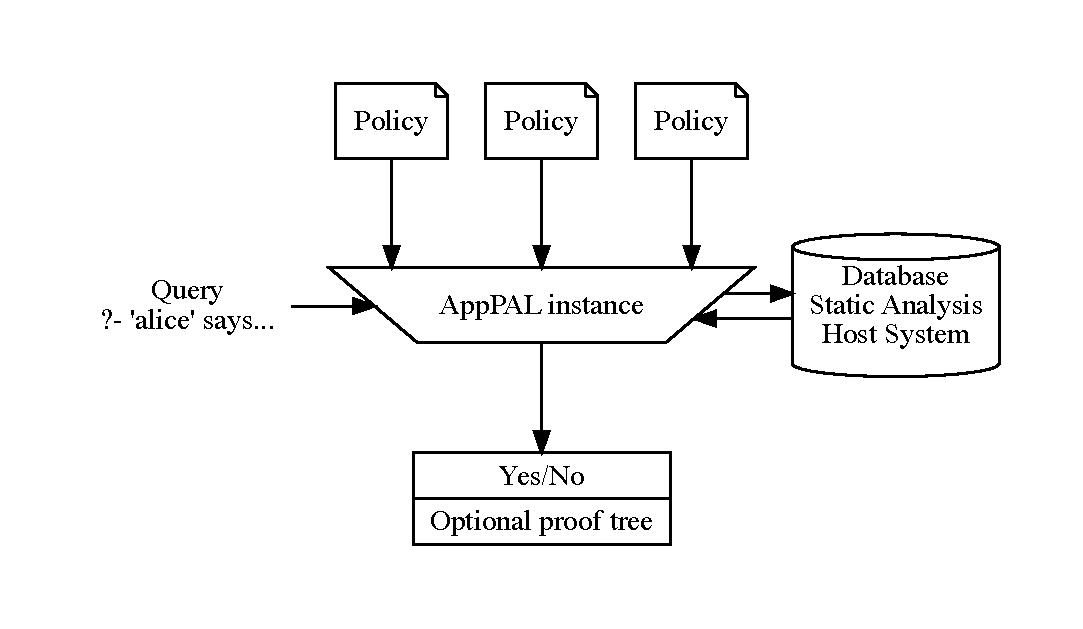
\includegraphics[width=\linewidth]{figures/apppal-evaluation.pdf}
  \caption{AppPAL's inputs and outputs.}
  \label{fig:apppal-inputs-outputs}
\end{figure}

\subsection{Evaluation}
\label{ssec:evaluation-alg}

Pseudo-code for the evaluation algorithm used by AppPAL is described
in~Figures~\ref{alg:eval1},~\ref{alg:eval2}~and~\ref{alg:eval3}.

To make queries against a policy, AppPAL is first given one or more policy files.
AppPAL parses the files and adds the assertions within them to the \ac{AC}. The
AC is then preprocessed to extract more information; this is summarised in
\autoref{tab:apppal-sets}. If a constant is used before a \emph{says} statement,
or it is used as the subject of a \emph{can-say} fact then the constant is
marked as \emph{voiced}. A constant is \emph{voiced} if it is the speaker of a
statement or it is the subject of a \emph{can-say} fact. A constant is a
\emph{subject} is it is the subject of a fact. The predicates used in the policy
are also extracted and marked as \emph{derivable}. This allows some queries to
be decided automatically and some rules to be flagged as unusable in the
assertion context. This lets AppPAL reject some queries quickly: if a query has
a speaker that isn't voiced then we cannot query what the speaker says. If a
rule relies on un-derivable predicates, then it cannot be used to make decisions.

A results table ($RT$) is also created. All ground facts in the assertion
context are added to the results table as proven facts. The table stores
partial results and previously established proofs. The table is indexed by
queries and a delegation depth, partial results (i.e. that the evaluation of
this query is ongoing). This allows previous results to reused without
re-computation or constraint re-evaluation. It also prevents AppPAL proofs
growing unboundedly (and the decision process not terminating). If when
searching for a proof we meet a query that we are currently evaluating,
i.e.~one that exists higher in the current proof tree, we treat it as false.
Multiple queries will share the same results table until the table is cleared,
or the AppPAL instance is stopped.

Ignoring queries we are currently evaluating lets us avoid proofs with cycles
(i.e. proof trees where the proof of a query depends on proving itself).  If we
can find a terminating proof with a cycle then we can find also shorter proof
by removing the cycle.  If a proof tree has a cycle that never terminates
(i.e.~it loops infinitely) then we can treat it as effectively false as it
would take an infinite amount of time to derive.

When evaluating the policy we also track which rules and predicates we have
used. From this we can reconstruct a proof tree that shows how AppPAL made a
decision. This allows an auditor to check the decision-making process and aids
AppPAL's developers with debugging.

\begin{table}
  \centering\sffamily\small
  \newcommand{\myset}[1]{\ensuremath{\text{\sffamily #1}}}
  \begin{tabular}{r l c}
    \toprule
    $c \in \myset{Voiced} \impliedby$     & $\exists \left(c \text{~says~} \cdots\right) \in \text{AC}$                        & $\bigvee$ \\
                                          & $\exists \left(\star \text{~says~} c \text{~can-say~} \cdots\right) \in \text{AC}$ &           \\
    $c \in \myset{Subjects} \impliedby$   & $\exists \left(\star \text{~says~} c\cdots\right) \in \text{AC}$                   & $\bigvee$ \\
                                          & $\exists \left(\cdots \text{~if~} \cdots,c~\star,\cdots\right) \in \text{AC},$     &           \\
                                          & $c \in \myset{Constants}$                                                          &           \\
    $p \in \myset{Derivable} \impliedby$  & $\exists \left( \cdots \star~p\left(\cdots\right) \cdots\right) \in \text{AC}$     &           \\
    \bottomrule                          \\
  \end{tabular}
  \caption{Sets used in AppPAL evaluation.}
  \label{tab:apppal-sets}
\end{table}

\begin{figure}\footnotesize\sffamily\centering
  \begin{algorithm}[H]
    \Fn(){\FnEvaluate{AC, RT, Q, D}}{
      \If{$RT$.\FnContains{(Q, D)}}{
        $result$ $\gets$ {$RT$.\FnGet{(Q, D)}}\;
        \If{result=Success}{
          \Return $result$
        }
        \Else{
          \Return{Failure}
        }
      }
      \Else{
        $RT$.\FnSet{(Q, D), (Inprogress, p)}\;
        $p$ $\gets$ \FnCond{AC, RT, Q, D}\;
        \If{p=Proven}{
          $RT$.\FnSet{(Q, D), Success}\;
          \Return{Success}\;
        }
        \Else{
          $p$ $\gets$ \FnCanSayCanActAs{AC, RT, Q, D}\;
          \If{p=Proven}{
            $RT$.\FnSet{(Q, D), Success}\;
            \Return{Success}\;
          }
          \Else{
            $RT$.\FnSet{(Q, D), Failure}\;
            \Return{Failure}\;
          }
        }
      }
    }
  \end{algorithm}
  \caption{Pseudo-code for evaluating a query.}
  \label{alg:eval1}
\end{figure}
\begin{figure}\footnotesize\sffamily\centering
  \begin{algorithm}[H]
    \Fn(){\FnCond{AC, RT, Q, D}}{
      \For{a $\in$ \FnAssertions{AC}}{
        $u$ $\gets$ $Q$.\FnUnify{a.\FnHead{}}\;
        \If{u.\FnValid{}}{
          $a$ $\gets$ $a$.\FnApply{u}\;
           \For{$\theta$ $\in$ \FnVarSubs{AC, a}}{
            $a^\prime$ $\gets$ $a$.\FnApply{$\theta$}\;
            \If{\FnVariables($a^\prime$) = $\emptyset$}{
              \If{$\forall$ b $\in$ a$^\prime$.\FnBody{}: \FnEvaluate{AC, RT, b, D}=Success}{
                \If{\FnCheckConstraint{a$^\prime$.constraint}=True}{
                  \Return{Success}
                }
              }
            }
          }
        }
      }
      \Return{Failure}
    }
  \end{algorithm}
  \caption{Pseudo-code for using the cond-rule.}
  \label{alg:eval3}
\end{figure}
\begin{figure}\footnotesize\sffamily\centering
  \begin{algorithm}[H]
    \Fn(){\FnCanSayCanActAs{AC, RT, Q, D}}{
      \For{c $\in$ \FnConstants{AC}}{
        \If{c $\in$ \FnSubjects{AC}}{
          \If{\FnCanActAs{AC, RT, Q, D, c} = $Proven$}{\Return{$Proven$}}
        }
        \If{D = $\infty$ $\wedge$ c $\in$ \FnSpeakers{AC}}{
          \If{\FnCanSay{AC, RT, Q, D} = $Proven$}{\Return{$Proven$}}
        }
      }
      \Return{Failure}
    }
   \; 
    \Fn(){\FnCanActAs{AC, RT, Q, D, c}}{
      $q_1 \gets$ $Q$.speaker \texttt{says} $c$ \texttt{can-act-as} $Q$.subject.\; 
      $q_2 \gets$ $Q$.speaker \texttt{says} $c$ $Q$.verbphrase.\;
      $p_1 \gets$ \FnEvaluate{AC, RT, $q_1$, D} = $Proven$\;
      $p_2 \gets$ \FnEvaluate{AC, RT, $q_2$, D} = $Proven$\;
      \If{$p_{1} \wedge p_{2}$}{\Return $Proven$}
      \Else{\Return $Failure$}
    }
   \; 
    \Fn(){\FnCanSay{AC, RT, Q, D, c}}{
      $q_{1\infty} \gets$ $Q$.speaker \texttt{says} $c$ \texttt{can-say inf} $Q$.fact.\; 
      $q_{2\infty} \gets$ c \texttt{says} $Q$.fact.\;
      $p_{1\infty} \gets$ \FnEvaluate{AC, RT, $q_1$, $\infty$} = $Proven$\;
      $p_{2\infty} \gets$ \FnEvaluate{AC, RT, $q_2$, $\infty$} = $Proven$\;
      $q_1 \gets$ $Q$.speaker \texttt{says} $c$ \texttt{can-say} $Q$.fact.\; 
      $q_2 \gets$ $c$ \texttt{says} $Q$.fact.\;
      $p_1 \gets$ \FnEvaluate{AC, RT, $q_1$, 0} = $Proven$\;
      $p_2 \gets$ \FnEvaluate{AC, RT, $q_2$, 0} = $Proven$\;
      \If{$(p_{1\infty} \wedge p_{2\infty})\vee(p_{1} \wedge p_{2})$}{\Return $Proven$}
      \Else{\Return $Failure$}
    }
  \end{algorithm}
  \caption{Pseudo-code for using the can-say and can-act-as rules.}
  \label{alg:eval2}
\end{figure}

AppPAL's evaluation procedure is not the same as SecPAL's, though in practice
both could be used to evaluate AppPAL or SecPAL policies.  SecPAL was evaluated
by first converting queries and policies into \datalogc{}.  Becker then
described a novel \datalogc{} evaluation algorithm with tabling to evaluate the
converted queries and make decisions. The AppPAL evaluation algorithm does not
make use of  \datalogc{}, but instead implements AppPAL's
evaluation rules directly.  We do, however, borrow some strategies from
Becker's SecPAL evaluation algorithm---AppPAL's results table serves a similar
purpose to SecPAL's tabling caching results and preventing cycles.  The use of
sets to restrict the search space for variables is unique to the AppPAL
algorithm, however. 

Our method for evaluating AppPAL offers an alternative to Becker's procedure.
We developed it to avoid having to implement \datalogc{}, and to allow us
greater control over how AppPAL evaluated policies.  We believe the procedure
is equivalent to Becker's SecPAL evaluation algorithm (though a more rigorous
comparison as to how the procedures compare has not been done).

\subsection{Soundness and Completeness of Decision Procedure}

The algorithm as described is neither sound nor complete as it makes
use of a results table $RT$, but has no means to invalidate results in
it. This causes problems when handling constraints, in particular
temporal ones.

Consider a constraint that states that the current time must be between
9~\textsc{am} and 3~\textsc{pm}. At 8:59~\textsc{am} we try to evaluate a query
that depends on this constraint being true (i.e. all possible proof trees use
this constraint). No proof can be found so the \texttt{Evaluate} function
correctly returns failure and the $RT$ is updated accordingly. At
9:01~\textsc{am} the query is re-run. Since a past result already exists in $RT$
it is reused and evaluate returns failure again, despite the constraint now
being satisfiable. Therefore, the algorithm is incomplete as it has failed to
find a proof when one exists. A similar argument for soundness can be made by
evaluating a query successfully at 2:59~\textsc{pm} and then again at
3:01~\textsc{pm}. A successful result may be returned which is unsound.

We use the results table to cache results, and to avoid circular proof
searches.  It helps makes the algorithm fast, albeit at the cost of soundness
and completeness. If AppPAL were incorporated into a production system, the
designers would need to have a strategy to manage the $RT$ and delete old
results. A simple strategy, such as clearing any statements older than 10
minutes, may be enough for most scenarios.  Alternatively the cache can be
cleared between queries, though this loses some of the speed benefits of having
some common sub-query results cached.  Ultimately the decision of how to manage
the results table is up to the developer.

The arguments in the rest of the section assume that the result of evaluating a
constraint does not change over time. This allows us to argue the
correctness of the algorithm, assuming that the $RT$ cache is correct.

When describing SecPAL Becker also showed that decision procedure he
used for SecPAL was both sound and complete.  His decision procedure
had to parts: a translation from SecPAL into \datalogc{}, and a
Datalog evaluation algorithm involving tabling.  He proved the
soundness and completeness of both parts in Appendix~C of the SecPAL
technical report~\cite{becker_secpal:_2006}.  To do so, he described
the SecPAL evaluation algorithm as a labelled transition system and
proved by induction which states were reachable from an initial state.
%
In comparison to Becker's proofs, the arguments presented here for
AppPAL work through induction on the height of the proof tree
generated by applying AppPAL's evaluation rules.
%
Becker did not have to consider constraints when presenting his proofs
as the SecPAL evaluation algorithm does not cache SecPAL queries.  It
does make use of a results table, but this stores the Datalog
translation of the SecPAL statement without constraint only, and so
the problems associated with the results of constraints changing over
time do not apply.

\subsubsection*{Soundness Argument}

\begin{equation*}
  \mathtt{Evaluate}(AC, RT, Q, D) = \textit{Success} \implies
  AC, D \models Q.
\end{equation*}


\paragraph*{Base Case.} For the base case we argue that the
\texttt{Evaluate} function is sound when not making recursive calls.
A query is \texttt{Evaluate}-d at a given delegation depth, against a
given $AC$ and $RT$. If the query has been made before, then the
result will be present in $RT$, and will be reused. Therefore, in
showing \texttt{Evaluate} is sound we must show that only queries that
can be proven are ever marked as successful in $RT$.

The \texttt{Evaluate} function calls \texttt{Cond} function which
implements SecPAL's \emph{cond} rule.  It searches the AC for unifying
assertions (i.e. those assertions which have a head that is equal to
the query under a variable renaming), then searches for possible
variable substitutions that remove all variables. If the body is missing
(i.e. the unifying assertion has no conditionals) and the constraint
is true, then \texttt{Cond} will return success, and the results table
will be updated accordingly.  This corresponds to SecPAL's \emph{cond}
rule (we have \fade{greyed out} the recursive case), hence we would
argue it is sound as there is no other means for our evaluation
algorithm to mark a result as true in $RT$ without recursively calling
\texttt{Evaluate}.  We call the call tree of \texttt{Evaluate} $T_{\mathtt{E}}^1$.

    The analogous proof tree to $T_{\mathtt{E}}^1$ (called
$T_{\models}^1$) produced by the evaluation rules, also relies on the
\emph{cond} rule (shown below with recursive elements \fade{greyed
out}).  Both $T_{\mathtt{E}}^1$ and $T_{\models}^1$ have height 1.

{\small
\begin{equation*}
  \infer[\textsf{\scriptsize cond}]{%
    AC, D \models A\texttt{~says~}fact\theta
  }{%
    \begin{array}[c]{c}
      \left(A\texttt{~says~}\text{fact}\fade{\texttt{~if~}\text{fact}_1,~\ldots,~\text{fact}_k}~\texttt{where}~c\right) \in AC \\
      \fade{AC,D\models A\texttt{~says~}\text{fact}_i\theta \; \forall i \in \{1\cdots k\}}
    \end{array}
    & \models{c\theta}
    & \textsf{vars}(\text{fact}\theta) = \emptyset)
  }
\end{equation*}
}

\paragraph*{Inductive Hypothesis.} Suppose we know that we know that
if \texttt{Evaluate(AC, $\{\}$, Q, D)} implies that $AC,D\models{Q}$,
where the height of the call tree of \texttt{Evaluate} is $n$ (in
calls of \texttt{Evaluate}), and that the height of the implied
derivation tree is also $n$.  We hypothesise that if \texttt{Evaluate}
is sound with a call tree and derivation tree height of $n$, then when
\texttt{Evaluate}'s call tree height is $n+1$, there will be an
equivalent derivation tree with height $n+1$.

\paragraph*{Inductive Step.}  Let $T_{\mathtt{E}}^n$ be the call tree
from a call to \texttt{Evaluate} with corresponding proof tree
$T_{\models}^n$, both with height $n$.  Let $T_{\mathtt{E}}^{n+1}$ be a
call tree of height $n+1$ where $T_{\mathtt{E}}^n$ is a child of the
root node. To show the hypothesis is true we must show that
however the \texttt{Evaluate} function proceeds, it must correspond to one
of AppPAL's evaluation rules; so the corresponding proof tree
$T_{\models}^{n+1}$ is the matching evaluation rule with $T_{\models}^n$
as (one of) its children.

We can ignore the results table (if it starts empty, or only contains
sound results) as it is just memoising results which could be
recalculated without memoisation.  We do not need to consider to the
case of non-terminating queries (i.e. circular), as \texttt{Evaluate}
will return \texttt{Failure} when the loop is detected.

\texttt{Evaluate} will call \texttt{Cond}, \texttt{CanSay} or
\texttt{CanActAs} each which implements the corresponding evaluation
rule and each of which calls \texttt{Evaluate}, where at least one
call of which will produce $T_{\mathtt{E}}^n$.  The corresponding
proof tree will have the equivalent evaluation rule at its root and
$T_{\models}^n$ as its child.  Therefore, $\mathtt{Evaluate}(AC, RT, Q,
D) = \textit{Success}$ implies we can always find an equivalent $AC, D
\models Q.$

\subsubsection*{Completeness Argument}

\begin{equation*}
  AC, D \models Q.
  \implies
  \mathtt{Evaluate}(AC, RT, Q, D) = \textit{Success} 
\end{equation*}

% Assume the RT is kept empty

\paragraph*{Base Case.}  Consider the case where a query has been
evaluated with AppPAL's evaluation rules and found true. Suppose the
height of proof tree used to derive it is 1, that is to say that we
have only used the \emph{cond} rule once to show the query is
valid. In this case the query must be unifiable with a fact in the AC
(i.e. one with no \emph{if} part).  If this is the case, when using
the \texttt{Evaluate} function we will call \texttt{Cond}, which will
search the AC for assertions to unify with.  Since (at least) one
assertion must exist (without an \emph{if}) for the \emph{cond} rule
to return true, then we will find it and \texttt{Evaluate} will always
also return \texttt{Success}, without recursively calling itself.

\paragraph*{Induction Hypothesis.}  Suppose know that for a proof
tree of a query $q$ (given an $AC$, and $D$) with height $n$, when running
\texttt{Evaluate(AC, $\{\}$, Q, D)} it will eventually return
\texttt{Success} (with at least $n$ recursive calls to
\texttt{Evaluate}).  We hypothesise that for a proof tree of height
$n+1$, \texttt{Evaluate} will also return success (given the same
$AC$ and $q$), with a recursive call depth of $n$.

\paragraph*{Inductive Step.}  The \texttt{Evaluate} function will (in
the worst case) search the entire $AC$ for a rule which will unify
with the currently evaluated query, and evaluate to \texttt{Success}.
We argue that evaluate implements each of the AppPAL evaluation rules
by comparison between the code and the inference rules.

For a proof tree of height $n+1$, where $n>0$, we will use one of the
\emph{cond}, \emph{can-say} or \emph{can-act-as} rules to derive the
proof tree at height $n$.  Each of the \texttt{Cond}, \texttt{CanSay},
and \texttt{CanActAs} functions which implement these evaluation rules
will call \texttt{Evaluate} at least once (corresponding to the
dependent proofs in the proof tree).  The induction hypothesis says
that these will be complete and will have at most $n$ recursive
calls to \emph{Evaluate}.  So at height $n+1$ the algorithm must be
complete as if the proof tree is valid, \texttt{Evaluate} would be
able to evaluate the corresponding assertions and with a call tree
height of $n+1$.

\subsection{Benchmarks}
\label{ssec:benchmarks}

Someone who uses AppPAL might wish it to check apps before installation. Since
policy checks may involve inspecting many rules and constraints one may ask
whether the checking will be acceptably fast. Downloading and installing an app
takes about 30 seconds on a typical Android phone over WiFi. If checking a
policy delays this even further a user may become annoyed and disable AppPAL.

A synthetic benchmark is used to give a measure AppPAL's performance. The policy
checking procedure is at its slowest when having to delegate repeatedly; the
depth of the delegation tree is the biggest reason for slowing the search.
Synthetic benchmarks checks that the checking procedure performed acceptably.
Each benchmark consisted of a chain of delegations. The \emph{1 to 1} benchmark
consists of a repeated delegation between all the principals. In the \emph{1 to
2} benchmark each principal delegated to 2 others and in the \emph{1 to 3}
benchmark each principal delegated to 3 others. These benchmarks are reasonable
as they model the slowest kinds of policies to test---though worse ones could be
designed by delegating even more or triggering an expensive constraint check.

\noindent
\begin{figure}\centering\footnotesize\sffamily
\begin{minipage}[t]{.32\textwidth}
\begin{lstlisting}[basicstyle=\ttfamily\footnotesize]
'0' says '1' can-say
  X isInstallable.
'1' says '2' can-say
  X isInstallable.
'2' says '3' can-say
  X isInstallable.
\end{lstlisting}
\end{minipage}\hfill
\begin{minipage}[t]{.32\textwidth}
\begin{lstlisting}[basicstyle=\ttfamily\footnotesize]
'2' says '4' can-say
  X isInstallable.
'2' says '5' can-say
  X isInstallable.
'3' says '6' can-say
  X isInstallable.
'3' says '7' can-say
  X isInstallable.
\end{lstlisting}
\end{minipage}\hfill
\begin{minipage}[t]{.32\textwidth}
\begin{lstlisting}[basicstyle=\ttfamily\footnotesize]
'4' says '12' can-say
  X isInstallable.
'4' says '13' can-say
  X isInstallable.
'4' says '14' can-say
  X isInstallable.
'5' says '15' can-say
  X isInstallable.
'5' says '16' can-say
  X isInstallable.
'5' says '17' can-say
  X isInstallable.
\end{lstlisting}
\end{minipage}
\caption{Excerpts from the 1~to~1, 1~to~2 and 1~to~3 benchmarks.}
\label{fig:benchmark-excerpts}
\end{figure}

For each benchmark we controlled the number of principals in the policy file:
as the number of principals increased so did the size of the policy.
The results are shown in \autoref{tab:benchmarks}.
Most typical policies (such as those discussed in \autoref{chap:apps-and-stores} and \autoref{chap:byod}), use only few delegations per decision.
We believe the policy checking performance of AppPAL is acceptable as unless a policy consists of hundreds of delegating principals the overhead of checking an AppPAL policy is negligible, even on a power constrained device such as a mobile phone.


\begin{table}
  \centering\sffamily\scriptsize\noindent
  \begin{minipage}{0.35\textwidth}
    \begin{tabular}{c c r@{.}l}
      \toprule
      Delegations & Principals & \multicolumn{2}{c}{Time (s)} \\
      \midrule
      1 to 1 & 10   &  0&01 \\
      1 to 1 & 100  &  1&00 \\
      1 to 1 & 500  & 20&90 \\
      1 to 1 & 1000 & 88&73 \\
      \midrule
      1 to 2 & 10   &  0&01 \\
      1 to 2 & 100  &  0&43 \\
      1 to 2 & 500  &  7&36 \\
      1 to 2 & 1000 & 27&47 \\
      \midrule
      1 to 3 & 10   &  0&01 \\
      1 to 3 & 100  &  0&24 \\
      1 to 3 & 500  &  3&99 \\
      1 to 3 & 1000 & 15&28 \\
      \bottomrule
    \end{tabular}
    \end{minipage}
    \begin{minipage}{0.64\textwidth}
    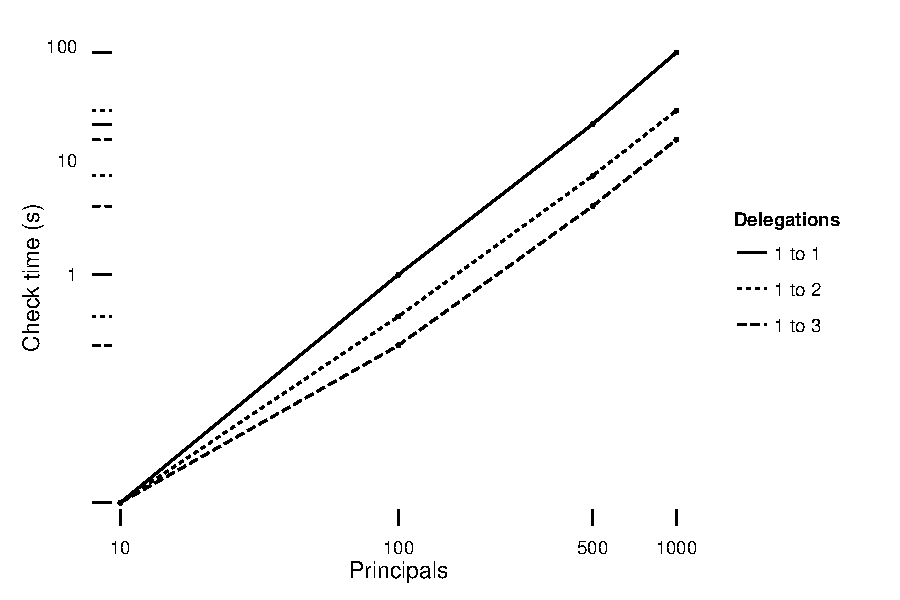
\includegraphics[width=\linewidth]{figures/benchmarks.pdf}
    \end{minipage}
  \caption{Benchmarking results on a Nexus 4 Android phone.}
  \label{tab:benchmarks}
\end{table}


\section{Automatic Analysis of AppPAL policies}
\label{sec:lint}

When examining an AppPAL policy it is natural to wonder whether the
policy is as optimal, in terms of the rules and facts required to
decide a query and the number of rules in the policy, as it could
be. Is a decision reachable given the rules and facts contained in the
policy?  Does an assertion context contain enough statements to use a
given rule? If there are multiple ways of deciding whether some
statement is true or not, does one rule require fewer statements than
any other? Does one rule require only a subset of the facts of another
rule, implying the second is redundant?

Policies can be checked for many properties including:
\begin{description}
\item[Satisfiability.] Do there exist rules which can never be satisfied?
\item[Equivalence.] Do there exist rules which have the require the same ground facts to be proven in order to satisfy them?
\item[Redundancy.] Do there exist multiple rules to make a decision where one is satisfied by a subset of the facts that satisfy the other?
\item[Consistency.] Can two contradictory decisions be made?
\end{description}

We have implemented preliminary checkers for two of these properties. The code
is included with AppPAL. The output shown in \framebox{\texttt{teletype}} is
output by the tools we have produced, and the diagrams shown in
\autoref{ssec:redundancy} are produced when running the tools in debug mode.
Additionally, a checker for \emph{consistency} could be implemented by using the
same technique as the Ponder authorization language and disallowing predicates
of the form \texttt{can$\star$} and
\texttt{cannot$\star$}~\cite{damianou_ponder_2001}.


\subsection{Checking Satisfiability}
\label{ssec:checking-satisfiability}

An assertion is \emph{satisfiable} if there are sufficient facts
such that the assertion's conditions can be met.
%
This is related to the concept of \emph{satisfiability} in SMT solving
(where a propositional logic formula is satisfiable if there is an
assignment of truth values to the propositional variables that makes
the formula true), but made more complex by the recursive nature of
AppPAL's (and other policy and database languages) assertions. Instead
of just looking for an assignment of variables, we must look to see if
there are rules and facts sufficient that we can derive the
satisfiable statement.

We care about this property when writing policies as it means that our
assertions affect something.  If an assertion is \emph{unsatisfiable,}
then this may indicate that we have failed to specify one of the
conditions it depends upon.

In Datalog (and, more generally, in logic programming) a Datalog
predicate, found by satisfying a rule, is satisfiable if there are
sufficient ground facts in the database to deduce it. Formally,
satisfiability in Datalog is defined in terms of the \ac{IDB} (the
Datalog \emph{program}, analogous to a policy file loaded into an
AppPAL assertion context), and the \ac{EDB} (a set of facts from both
the \ac{IDB} and those which can be derived using rules).
Satisfiability for Datalog is defined
as~\cite{alon_levy_equivalence_1993}:

\begin{quote}
  \textbf{Satisfiability:} An IDB predicate $s$ of a program $P$ is
  \emph{satisfiable} if there is some EDB $D$, such that $P$ defines a
  non-empty relationship for $s$.
\end{quote}

In AppPAL, when an assertion is satisfiable, there is a combination of
facts that could satisfy its conditionals. If there are no facts that
could ever satisfy the rule, then the policy may have a bug. An
analogy can be drawn to an \emph{conditional always false bug} in a
conventional programming language: we have code (or in this case a
rule) that can never be used as the conditions for using it can never
occur.

Drawing from the Datalog definition of satisfiability, we define an
AppPAL statement $G$ as satisfiable if there exists some \ac{AC} such
that there is an assertion $A$ within the AC and some assignment of
variables $\theta$ such that $A\theta$ derives $G$, and that all the
conditions in the body of $A\theta$ are also satisfiable.  Formally,
we define this as:
%
\begin{align*}
  G \in \text{Satisfiable}~\text{\textit{if}}~\exists A \in \text{AC}:~&\exists \theta:~G\equiv\text{head}(A\theta) \\
                                                              \wedge~ & (\text{conditionals}(A) = \emptyset \\
                                                                      & \vee~\forall G^\prime \in \text{conditionals}(A\theta).~G^\prime \in \text{Satisfiable}.)
\end{align*}

Our satisfiability checker works by examining which assertions each
principal could possibly say from a given assertion context.  When
checking the satisfiability we ask whether there is a mechanism in the
policy for the principal to use a given predicate.
We use the following
rules with a relaxed notion of $\in$, that allows variable unification:

\begin{center}\footnotesize
  \begin{equation*}
\infer[(1)]{
  AC\vdash (\text{\tt principal}, \text{\tt predicate})\in \text{Satisfiable}
}{
  \begin{array}{c}
  \exists A \in AC~s.t.~A\equiv\left( \text{\tt principal says $\star$ predicate if $\star~p_1,~\cdots,~\star~p_n$.} \right) \\
  \forall p \in \left( p_i\cdots p_n \right):~AC\vdash(\text{\tt principal}, p) \in \text{Satisfiable}
  \end{array}
}
  \end{equation*}
  
  \begin{equation*}
\infer[(2)]{
  AC\vdash (\text{\tt principal}, \text{\tt predicate})\in \text{Satisfiable}
}{
  \begin{array}{c}
  \exists A \in AC~s.t.~A\equiv\left( \text{\tt principal says $\star$ $S$ can-say predicate if $\star~p_1,~\cdots,~\star~p_n$.} \right) \\
  \forall p \in \left( p_i\cdots p_n \right):~AC\vdash(\text{\tt principal}, p) \in \text{Satisfiable} \\
  AC\vdash(S, \text{\tt predicate}) \in \text{Satisfiable}.
  \end{array}
}
  \end{equation*}
\end{center}

Informally the rules say when a policy (in an assertion context) supports the notion that a principal can say a predicate (that (\texttt{principal},~\texttt{predicate})~$\in$~Satisfiable).  Rule (1) says that a principal can make statements using a predicate if the assertion context contains an example of them doing so; and that if that example has conditionals, they policy also supports them saying each conditional's predicate.
Rule (2) handles the case with delegation:  a principal can use a predicate (that (\texttt{principal},~\texttt{predicate})~$\in$~Satisfiable), if they say someone else can say the predicate, and the policy supports the other person being able to use that predicate (that (S,~\texttt{predicate})~$\in$~Satisfiable)).

\pagebreak
To give an example, if we have an assertion context with the following assertions:
\begin{lstlisting}
'alice' says 'bob' recommends('angry-birds').

'alice' says 'claire' canInstall(App)
  if 'bob' recommends(App).

'alice' says 'claire' mustInstall(App)
  if 'bob' highlyRecommends(App).  
\end{lstlisting}
\noindent The first assertion can be used to show that:
$$(\text{\tt 'alice'},\text{\tt recommends('angry-birds')}) \in \text{Satisfiable}$$
\noindent The assertion is present in the policy and there are no conditions, so:
$$(\text{\tt 'alice'},\text{\tt recommends('angry-birds')}) \in \text{Satisfiable}$$

\noindent The second assertion shows that:
$$(\text{\tt 'alice'},\text{\tt canInstall(App)}) \in \text{Satisfiable}$$
\noindent In the second case we have a condition, but since the first assertion showed that:
$$(\text{\tt 'alice'},\text{\tt recommends('angry-birds')}) \in \text{Satisfiable}$$
\noindent Then we allow (with the relaxed notion of $\in$) that:
$$(\text{\tt 'alice'},\text{\tt recommends(App)}) \in \text{Satisfiable}$$

\noindent Finally the third assertion cannot be used to show that:
$$(\text{\tt 'alice'},\text{\tt mustInstall(App)}) \in \text{Satisfiable}$$
\noindent As we have no way to show that:
$$(\text{\tt 'alice'},\text{\tt highlyRecommends(App)})$$

We also add a somewhat weaker notion of satisfiability (Satisfiable$^\star$) which distinguishes
statements that might be satisfiable, but depend on delegation, and where the
delegated party has made no assertions about this predicate. This distinguishes
the case where we have missing information from the case where a speaker has
made an assertion that is itself unsatisfiable.

\begin{center}\footnotesize
  \begin{equation*}
\infer{
  AC\vdash (\text{\tt principal}, \text{\tt predicate})\in \text{Satisfiable*}
}{
  \begin{array}{c}
  AC\vdash (\text{\tt principal}, \text{\tt predicate})\not\in \text{Satisfiable} \\
  \exists A \in AC~s.t.~A\equiv\left( \text{\tt principal says $\star$ predicate if $\star~p_1,~\cdots,~\star~p_n$.} \right) \\
  \forall p \in \left( p_i\cdots p_n \right):~AC\vdash(\text{\tt principal}, p) \in \text{Satisfiable} \vee (\text{\tt principal}, p) \in \text{Satisfiable}^\star \\
  \exists p \in \left( p_i\cdots p_n \right):~AC\vdash(\text{\tt principal}, p) \in \text{Satisfiable}^\star \wedge (\text{\tt principal}, p) \not\in \text{Satisfiable}
  \end{array}
}
  \end{equation*}

  \begin{equation*}
\infer{
  AC\vdash (\text{\tt principal}, \text{\tt predicate})\in \text{Satisfiable}^\star
}{
  \begin{array}{c}
  \exists A \in AC~s.t.~A\equiv\left( \text{\tt principal says $\star$ $S$ can-say predicate if $\star~p_1,~\cdots,~\star~p_n$.} \right) \\
  \forall p \in \left( p_i\cdots p_n \right):~AC\vdash(\text{\tt principal}, p) \in \text{Satisfiable} \\
  \not\exists A \in AC~s.t.~A\equiv\left( \text{\tt $S$ says $\star$ predicate $\cdots$.} \right) 
  \end{array}
}
  \end{equation*}
\end{center}

The satisfiability rules are reminiscent of AppPAL's \emph{cond} and
\emph{can-say} rules shown in \autoref{fig:secpal-rules}, but far more
general.  AppPAL's evaluation rules decide if a specific assertion by
a speaker is supported by an assertion context.  In contrast, the
satisfiability rules look at whether it is possible that the
evaluation rules \emph{could} decide that the assertion is
supported---that the AppPAL evaluation rules could conceivably be
satisfied, not that the evaluation rules are satisfied for a specific
assertion.
  
This definition of satisfiability is not complete (it ignores relationships
formed using \emph{can-act-as}, as well as delegations to principals specified
as variables). It is, however, useful as a debugging tool as it can quickly
check that a policy contains enough statements to make any decision.

For a real example of the satisfiability checker in use, consider the following snippet taken
from the NHS policy described in \autoref{chap:byod}.  The rule
described in the policy is that an app must be approved by the
\ac{IGC} as well as by either the \ac{CACPG} as well as the \ac{MIG}
depending on whether it is for clinical or business use. We describe
this in AppPAL as:

\begin{lstlisting}
'nhs-trust' says App isInstallable
  if App isApproved, App isUsableClinically.
'nhs-trust' says App isInstallable
  if App isApproved, App isUsableNonClinically.
'nhs-trust' says 'igc' can-say App:isApproved.
'nhs-trust' says 'cacpg' can-say App:A isUsableClinically.
'nhs-trust' says 'mig' can-say App:A isUsableNonClinically.
\end{lstlisting}

What apps in practice are approved for use?
As the policy document notes, none of the groups or committees have ever
approved an app in practice.
When running the satisfiability checker on this policy,
it reports that (among other information) no app is installable.

\noindent\begin{minipage}{\textwidth}\vspace{1em}
\begin{lstlisting}
$\$$ java -jar Lint.jar --satisfiability example.policy
[INFO]: loaded 1/1 files of 6 assertions
Issues identified when checking satisfiability.
The following decisions may be unsatisfiable by their speakers:
'nhs-trust' says * isUsableClinically
'nhs-trust' says * isInstallable
'nhs-trust' says * isApproved
'nhs-trust' says * isUsableNonClinically

In particular the following assertions are unsatisfiable:
'nhs-trust' says App isInstallable if App isApproved, App isUsableNonClinically.
'nhs-trust' says App isInstallable if App isApproved, App isUsableClinically.

These decisions may be satisfiable through delegation but we
lack any statements to that effect from the delegated party:
(via 'cacpg') 'nhs-trust' says * isUsableClinically
(via 'igc') 'nhs-trust' says * isApproved
(via 'mig') 'nhs-trust' says * isUsableNonClinically
\end{lstlisting}
\end{minipage}

As well as reporting which decisions it cannot make, it also reports the
specific assertions as well. It also reports the assertions that may be
satisfiable through delegation given additional statements (the
Satisfiable$^\star$) separately at the bottom.

These checks are simple and we don't take into
account dependencies between variables. If we add, for example, the statements:

\begin{lstlisting}
'igc' says 'angry-birds' isApproved.
'cacpg' says 'dropbox' isUsableClinically.
'mig' says 'instagram' isUsableNonClinically.
\end{lstlisting}

Then we will still never find any installable apps, as the \ac{IGC}, \ac{CACPG}
and \ac{MIG} need to agree on the same app to find it installable. Our rules for
determining what is satisfiable only concern themselves with the predicates and
the principals: no checks are done to ensure that the subjects of the policies,
match up. In part this is because AppPAL has a closed-world assumption: if a
principal does not talk about a specific constant with respect to a predicate
then it is assumed false. When we run the satisfiability checker, we find no
problems as all the decisions are now satisfiable as there is a decision about
\emph{some} variable; even if that variable isn't useful in practice.

\noindent\begin{minipage}{\linewidth}\vspace{1em}
\begin{lstlisting}
$\$$ java -jar Lint.jar --satisfiability example.policy
[I]: loaded 1/1 files of 11 assertions
[I]: no satisfiability problems
\end{lstlisting}
\end{minipage}

The satisfiability checker acts as a quick sanity checker that a policy contains
enough facts and assertions; unlike AppPAL-proper which can check how and
whether a specific statement would be made.  

%The code in \autoref{alg:reachable} produces a set of pairs of predicates and
%speakers where the pair of a speaker and a predicate indicates that that
%speaker may say something about that predicate. We search over all the
%assertions in the AppPAL assertion context. If all of an assertion's
%conditionals (the facts in the if part) are reachable (or it has none) then the
%speaker and predicate are added to the reachable set. If the statement is a
%can-say statement then we additionally check if the delegated predicate is
%reachable from the delegated speaker, and if so mark the delegated statement as
%reachable from the speaker who made the can-say statement.
%
%\begin{lstlisting}[language=Python,float,caption={Procedure for finding all reachable assertions.},label={alg:reachable}]
%def reachable(ac) -> set:
%  reachable = new set()
%  iterate = True
%  while iterate == True:
%    iterate = False
%    for assertion in ac:
%      e = a.speaker
%      p = a.predicate
%      if p.isCanSay() and (e, p) in reachable:
%        if (p.delegator, p.delegation) in reachable:
%          if for all c in a.conditions: (e, c.predicate) in reachable:
%            reachable.add((e, p.delegation))
%            iterate = True
%      else if not (e, p) in reachable:
%        if for all c in a.conditions; (e, c.predicate) in reachable:
%          reachable.add((e, p))
%          iterate = True
%  return reachable
%\end{lstlisting}

\subsection{Checking Redundancy}
\label{ssec:redundancy}

If unsatisfiability can be caused when we lack sufficient facts and assertions
to make a decision then redundancy occurs when we have too many. Specifically
there are two types of redundancy~\cite{alon_levy_constraints_1992} that we care
about here:

\begin{itemize}
\item \emph{Unreachability} occurs if a predicate does not take part in the
  minimal derivation tree of a fact.
\item \emph{Irrelevance} occurs if a derivation tree contains pairs of identical atoms.
\end{itemize}

These ideas can be applied to AppPAL to detect some potential problems in AppPAL policies. For instance,  consider the
following AppPAL policy:

\begin{lstlisting}
'alice' says App isInstallable
  if App isRecommended,
     App isNotMalware.

'alice' says App isRecommended
  if App isNotMalware,
     App isGood.
\end{lstlisting}

Alice checks that the app is not malware when checking the app is
installable and when checking that the app is recommended.  The check
in \texttt{isInstallable} is irrelevant as it depends on the app being
recommended which also checks this property.  When writing AppPAL
policies this kind of irrelevance commonly occurs when using the
typed-syntax described in \autoref{ssec:types}. For example, in this
excerpt from a SANS BYOD policy there is a check that \emph{U} is a
user in both assertions.  In the first there is irrelevance because
\emph{U} is stated as being a user twice, where once would have been
sufficient.  In the second there is a single check that \emph{U} is a
user but it is irrelevant as the check had already been done when
checking if \emph{U} had lost the device (since only users can lose
devices in the first assertion).

\begin{lstlisting}
'company' says User:U can-say User:U hasLost(Device:D)
  if D isOwnedBy(U).

'company' says User:U mustInform('help-desk', 'device-lost')
  if U hasLost(Device).
\end{lstlisting}

Whilst the irrelevance adds redundancy and can slow down inferences when making policy checks, it can also aid policy comprehension.  In the previous example the repeated checks as to whether someone is a user do not, strictly, need to be done.  They do, however, clarify what the type of each variable is.  A future implementation of AppPAL might incorporate code to remove the redundant checks automatically.  In order to remove the redundant checks we must first be able to identify them, however.

We can check for irrelevance by building a proof-graph for the
assertion context.  Every node (shown in a box) represents an AppPAL fact we
might wish to prove.  For every assertion in the context we create a proof
(represented as a number in brackets) for the head of the assertion, which is
connected to the facts required to prove the assertion.  In the case of can-say
and can-act-as statements we expand them as per AppPAL's inference rules.
A proof-graph for the above example is shown in \autoref{fig:irrelevance}: the
irrelevant links are shown in red and the AppPAL facts connected to the two
dashed ones can be removed to remove the irrelevance.

\begin{figure}
  \centering
  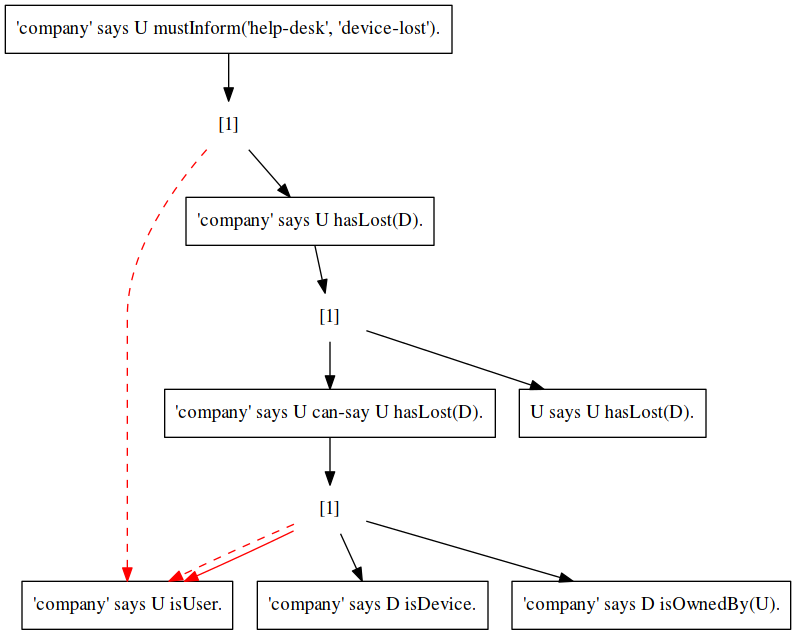
\includegraphics[width=0.5\linewidth]{./figures/irrelevance.png}
  \caption{Proof graph showing irrelevance.}
  \label{fig:irrelevance}
\end{figure}

In contrast, unreachability occurs when a fact does not take part in the minimal
derivation tree of a fact.  As a simple example consider the following policy:

\begin{lstlisting}
'alice' says App isInstallable if App isNotMalware.
'alice' says App isInstallable if App isNotMalware,  App isRecommended.
\end{lstlisting}

To detect unreachability for a given policy we again build the proof-graph (shown
in \autoref{fig:unreachability}).  For each proof node we collect the facts
(the leaves of the graph underneath it, which are the ground assertions from the
AC\footnote{Or in the case of an unsatisfiable policy facts with variables that
  cannot be unified with a ground fact.} in
AppPAL).  If the facts for one proof node connected to a fact are a subset of
the facts for another proof node, then the larger proof node is unreachable as it
contains facts which are not in the minimal derivation tree.   In the case of
\autoref{fig:unreachability}, the derivation-graph 2 is made redundant by
derivation-graph 1 as it contains a subset of the facts.  This is a
simplified example; in general facts lower in the tree may have multiple
derivation trees, leading to multiple sets of facts being required for a fact
that seems to have only one proof node.  Loops can also occur (where one fact
depends on itself to prove itself).  This approach isn't complete, but it does
identify several cases where an AppPAL policy may be redundant through
unreachability.


\begin{figure}
  \centering
  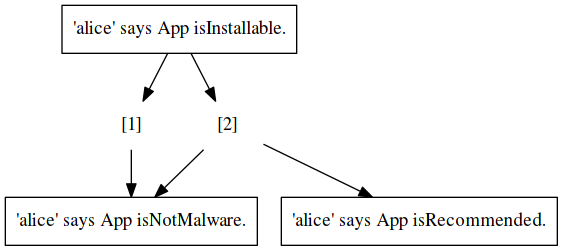
\includegraphics[width=0.5\linewidth]{./figures/unreachability.png}
  \caption{Proof graph showing unreachability.}
  \label{fig:unreachability}
\end{figure}

Redundancy can also occur when there are multiple rules that result in the
same decision being made.  Rules may depend on other rules, or ground
facts.  One proof ($A$) is made redundant by another proof ($B$) if
the set of ground facts used in $B$ is a subset of the ground facts
used in $A$. Whenever $A$ is satisfied $B$ will also be, but when $B$
is satisfied $A$ may not be: consequently $A$ is redundant as $B$ can
be used to prove its goal with fewer facts.  Informally, for any goal
$G$:
\begin{align*}
  \exists p_1 \in \text{proofs}(G).~\exists p_2 \in \text{proofs}(G).        & \\
  p_1 \not= p_2~\wedge~\text{facts}(p_1) \subset \text{facts}(p_2)           & \implies G\text{ has unreachable proofs.} \\
  p_1 \not= p_2~\wedge~\text{facts}(p_1) = \text{facts}(p_2)                 & \implies G\text{ has equivalent proofs.}
\end{align*}
Where $\text{proofs}(G)$ is the set of all possible proof trees for a goal $G$.

Additionally, if two different goals ($G$ and $G^\prime$) have
equivalent proofs, i.e. there are multiple proofs that both rely on the same ground facts, then we report this as it implies the two
statements may not be independent.
\begin{align*}
  \exists p_1 \in \text{proofs}(G).~\exists p_2 \in \text{proofs}(G^\prime). & \\
  \text{facts}(p_1) = \text{facts}(p_2)                                      & \implies \text{$G$ and $G^\prime$ have equivalent proofs.}
\end{align*}

A simple example might be the policy shown in \autoref{fig:redundancy-graph-simple}.
The second rule makes the first redundant.  We can represent the policy
as a graph shown opposite the policy.  The goal (shown as a blue rectangle) has two routes
to prove it true (each shown in ellipses).  Route 1 requires that the facts
(shown in green rectangles) \lstinline!'x' says 'y' r,! and
\lstinline!'x' says 'y' q.!, whereas route 0 only requires the
latter fact.

\begin{figure}
  \centering
  \begin{minipage}{0.4\linewidth}
    \begin{lstlisting}
'x' says 'y' p
  if 'y' q,
     'y' r.

'x' says 'y' p
  if 'y' q.
    \end{lstlisting}
  \end{minipage}
  \begin{minipage}{0.59\linewidth}
    \scriptsize{}\centering
    \def\svgwidth{\columnwidth}
    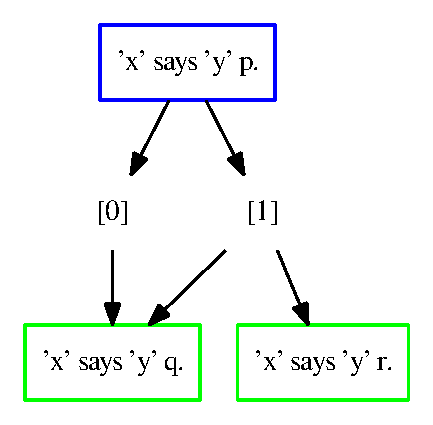
\includegraphics[width=0.59\linewidth]{figures/redundancy-simple.eps}
  \end{minipage}
  \caption{A simple policy shown as a graph.}
  \label{fig:redundancy-graph-simple}
\end{figure}

A more complex example is shown below:

\begin{lstlisting}
'x' says 'z' p if 'z' q.
'x' says 'y' can-say 'z' p.
'y' says 'z' p if 'z' q.
'y' says 'x' can-say 'z' q.
\end{lstlisting}

Representing this policy as the graph in \autoref{fig:redundancy-complex} we can see it is more complex. Goals that
depend on more than just green facts, are shown as black rectangles.  If a goal
is used to prove another goal, and it itself only depends on green, ground,
facts, then the node is marked to be flattened (red rectangle).  Its proofs are
merged into the higher proof, and the flattened goal is removed from the higher
proof.  This process is repeated until no more nodes can be flattened (shown
twice in \autoref{fig:redundancy-complex}).  Once the graph is flattened we can
identify that \lstinline!'x' says 'z' p! has a redundant means of proof (route
0 only uses one of route 1's facts).  We can also see that all the proofs for
\lstinline!'y' says 'z' q! and \lstinline!'y' says 'z' p! use the same facts.
We report these statements as having equivalent proofs as the goals are not
independent of each other (implying we could use fewer goals and still write
equivalent policies).

\begin{figure}
  \centering\tiny\noindent
  \hspace{2.5em}
  \framebox{\def\svgwidth{0.33\linewidth}1.
    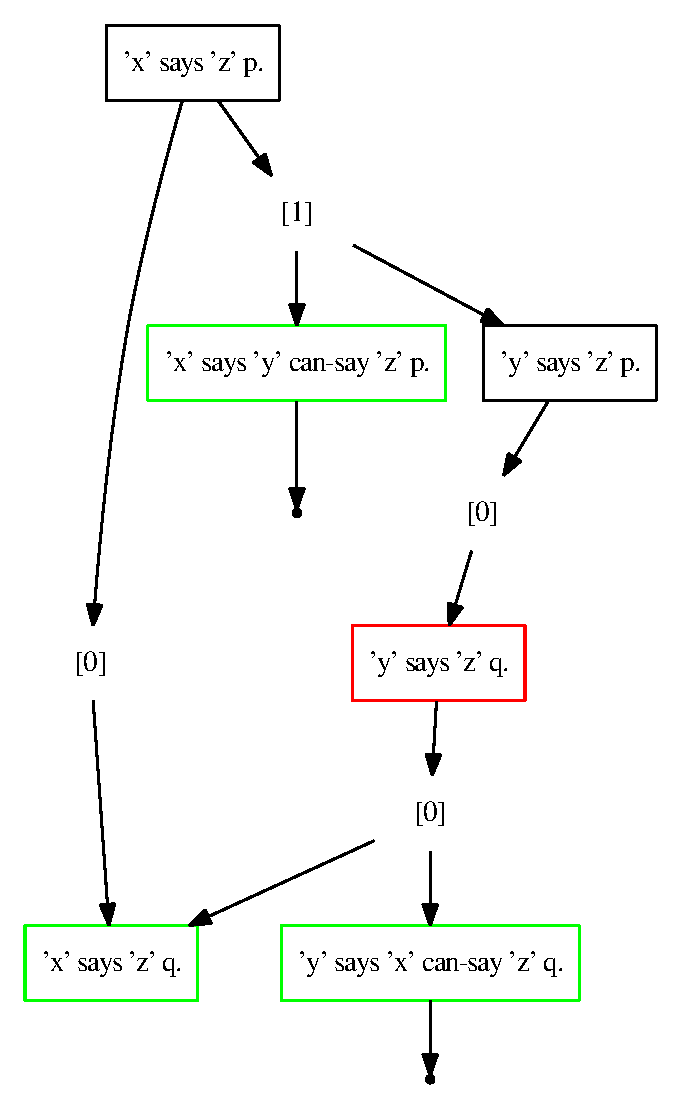
\includegraphics[width=0.33\linewidth]{figures/redundancy-complex-0.eps}}
  \framebox{\def\svgwidth{0.44\linewidth}2.
    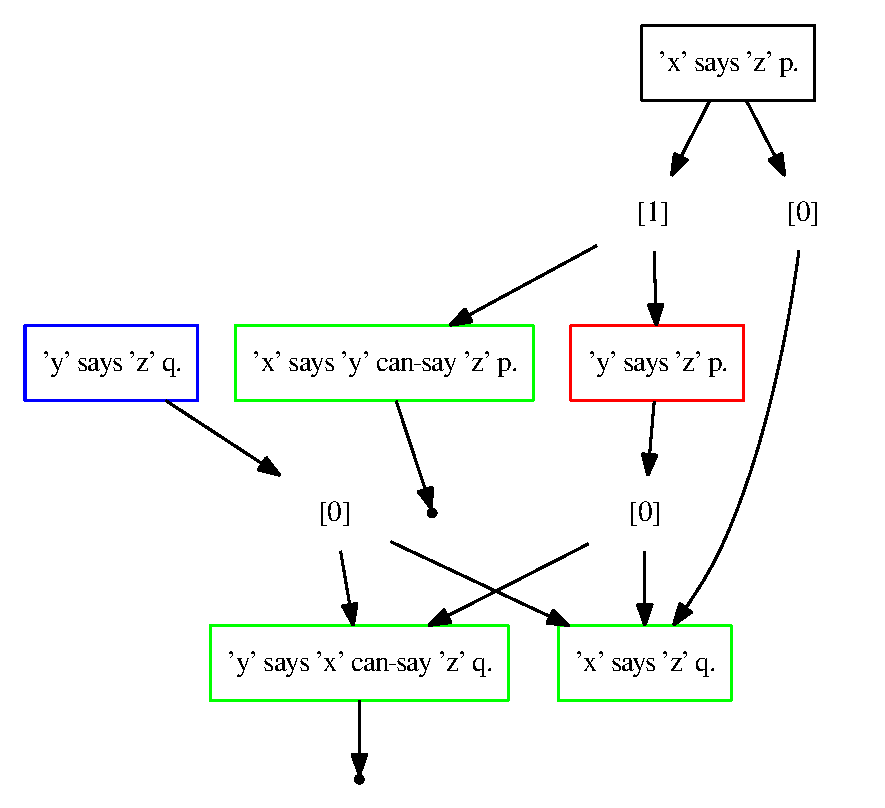
\includegraphics[width=0.44\linewidth]{figures/redundancy-complex-1.eps}}
  \newline\noindent
  \framebox{\def\svgwidth{0.8\linewidth}3.
    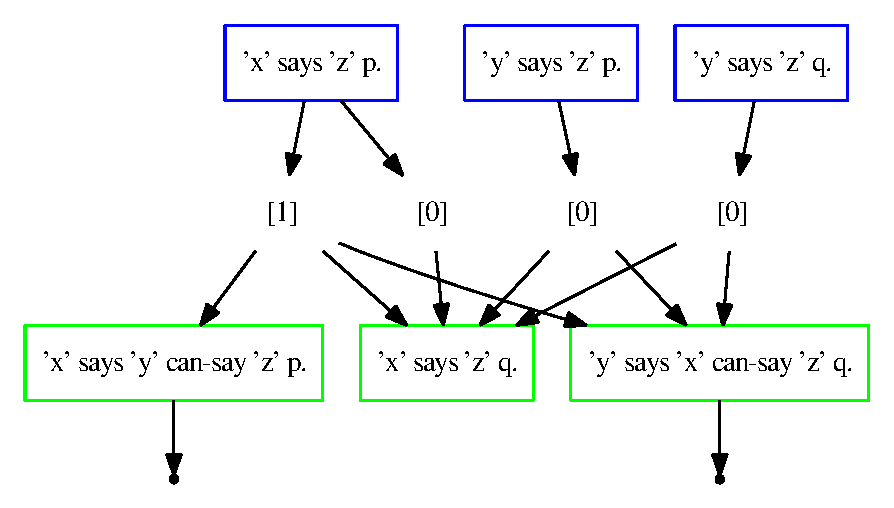
\includegraphics[width=0.8\linewidth]{figures/redundancy-complex-2.eps}}
  \caption{Flattening a more complex policy.}
  \label{fig:redundancy-complex}
\end{figure}

\end{document}

% vim: set makeprg=make\ ch3.pdf:

%%% Local Variables:
%%% mode: latex
%%% TeX-master: "../thesis"
%%% End:
